\documentclass[oneside,11pt]{book}

\usepackage{amsmath}
\usepackage{amsfonts}
\usepackage{hyperref}
\usepackage{amssymb,amsthm}
\usepackage[utf8]{inputenc}
%\usepackage{inconsolata}
%\usepackage[sc]{mathpazo}
\usepackage{newtxtext}
\usepackage{newtxmath}
\usepackage[scaled=.8]{sourcecodepro}
\usepackage{listings}

% Define Language
\lstdefinelanguage{futhark}
{
  % list of keywords
  morekeywords={
    do,
    else,
    fn,
    for,
    fun,
    if,
    in,
    include,
    let,
    loop,
    struct,
    then,
    type,
    val,
    while,
    with,
  },
  sensitive=true, % keywords are not case-sensitive
  morecomment=[l]{--}, % l is for line comment
  morecomment=[s]{\{-}{-\}}, % s is for start and end delimiter
%  otherkeywords={>,<,=,<=,>=,!,*,/,-,+,|,&,||,&&,==,=>},
  morestring=[b]" % defines that strings are enclosed in double quotes
}

% Define Colors
\usepackage{color}
\definecolor{eclipseBlue}{RGB}{42,0.0,255}
\definecolor{eclipseGreen}{RGB}{63,127,95}
\definecolor{eclipsePurple}{RGB}{127,0,85}

% Set Language
\lstset{
  language={futhark},
  basicstyle=\ttfamily, % Global Code Style
  captionpos=b, % Position of the Caption (t for top, b for bottom)
  extendedchars=true, % Allows 256 instead of 128 ASCII characters
  tabsize=2, % number of spaces indented when discovering a tab
  columns=fixed, % make all characters equal width
  keepspaces=true, % does not ignore spaces to fit width, convert tabs to spaces
  showstringspaces=false, % lets spaces in strings appear as real spaces
  breaklines=true, % wrap lines if they don't fit
  frame=trbl, % draw a frame at the top, right, left and bottom of the listing
  frameround=tttt, % make the frame round at all four corners
  framesep=4pt, % quarter circle size of the round corners
  numbers=left, % show line numbers at the left
  numberstyle=\small\ttfamily, % style of the line numbers
  commentstyle=\slshape\bfseries\color{eclipseGreen}, % style of comments
  keywordstyle=\bfseries\color{eclipsePurple}, % style of keywords
  stringstyle=\color{eclipseBlue}, % style of strings
  emph=[1] {
    abs,
    copy,
    concat,
    empty,
    false,
    filter,
    iota,
    map,
    partition,
    rearrange,
    reduce,
    reduceComm,
    replicate,
    reshape,
    rotate,
    shape,
    signum,
    scan,
    split,
    transpose,
    true,
    unzip,
    write,
    zip,
    zipWith,
  },
  emphstyle=[1]{\color{eclipseBlue}},
}

\newcommand{\sem}[1]{[\![#1]\!]}
\newcommand{\seme}[1]{\sem{#1}\varepsilon}
\newcommand{\semzero}[1]{\sem{#1}_0}

\newcommand{\emptymap}{\{\}}
\newcommand{\fracc}[2]{\begin{eqnarray} \frac{\begin{array}{c} #1
    \end{array}}{\begin{array}{c} #2 \end{array}} \end{eqnarray}}
\newcommand{\sembox}[1]{\hfill \normalfont \mbox{\fbox{\(#1\)}}}
\newcommand{\sempart}[2]{\subsubsection*{\rm\em #1 \sembox{#2}}}
\newcommand{\axiom}[1]{\begin{eqnarray} \begin{array}{c} #1 \end{array} \end{eqnarray}}
\newcommand{\fraccn}[2]{\refstepcounter{equation}\mbox{$\frac{\begin{array}{c} #1 \end{array}}{\begin{array}{c} #2 \end{array}}$}~(\arabic{equation})}
\newcommand{\fraccc}[2]{\mbox{$\frac{\begin{array}{c} #1 \end{array}}{\begin{array}{c} #2 \end{array}}$}}
\newcommand{\onepart}[1]{\noindent\hfill#1\hfill~\vspace{2mm}}
\newcommand{\twopart}[2]{\noindent\hfill#1\hfill#2\hfill~\vspace{2mm}}
\newcommand{\threepart}[3]{\noindent\hfill#1\hfill#2\hfill#3\hfill~\vspace{2mm}}
%\newcommand{\axiomm}[1]{\refstepcounter{equation}\mbox{$\begin{array}{c} #1 \end{array}$}~(\arabic{equation})}
\newcommand{\axiomm}[1]{$\begin{array}{c} #1 \end{array}$}
%\newcommand{\ar}[1]{\stackrel{#1}{\longrightarrow}}
\newcommand{\vd}{\vdash}
\newcommand{\Ran}{{\rm Ran}}
\newcommand{\Dom}{{\rm Dom}}
\newcommand{\kw}[1]{\texttt{#1}}
\newcommand{\id}[1]{\mbox{\it{#1}}}
\newcommand{\rarr}{\rightarrow}
\newcommand{\larr}{\leftarrow}

%\usepackage{xcolor}
\usepackage{tikz}

\newcommand{\size}{\ensuremath{\mathrm{size}}}
\renewcommand{\log}{\ensuremath{\mathrm{log}}}

\newtheorem{proposition}{Proposition}

% Avoid breaking lstlistings environments across pages.
\BeforeBeginEnvironment{lstlisting}{\vspace{\topskip}\par\noindent\begin{minipage}{\linewidth}}
\AfterEndEnvironment{lstlisting}{\end{minipage}\par}
\newenvironment{wrap}{\vspace{\topskip}\par\noindent\begin{minipage}{\linewidth}}{\end{minipage}\par}
\newcommand{\inplisting}[1]{\begin{wrap}\lstinputlisting{#1}\end{wrap}}
\newcommand{\pp}{+\!\!\!+}

\title{\bf Parallel Programming in Futhark}
\author{Troels Henriksen, Martin Elsman, and Cosmin E. Oancea \\[2mm] HIPERFIT \\[2mm] Department of Computer Science \\ University of Copenhagen (DIKU)}
\date{\today \\[5mm] Edition \\ 0.6}

\begin{document}
\frontmatter
\maketitle
\chapter{Preface}

This book is written with the aim of providing an introduction to
parallel functional programming and algorithms with the focus on using
the Futhark language as the development language.

Futhark is currently being actively developed but it is mature enough
that simple algorithms---and also quite a few non-trivial ones---can
be written in the language and executed in parallel on real parallel
GPU hardware.

The book is Open Source, maintained on github, and distributed under
the Creative Commons Attribution (By) 4.0 license. All code snippets
in the book, including code in the book's repository directory is
distributed under the MIT license. We will appreciate pull-requests
for fixing any kinds of typos and errors in the text and in the
enclosed programs. The book's main repository is \url{https://github.com/HIPERFIT/futhark-book}.

Regarding errors in the programs, most of the
programs written in the book can be run and tested against an expected
result; this execution and test can be done by typing \texttt{make} in
the \texttt{src/} directory of the repository.

\section*{Acknowledgments}
This work has been partially supported by the Danish Strategic Research
Council, Program Committee for Strategic Growth Technologies, for the
research center HIPERFIT: Functional High Performance Computing for
Financial Information Technology (\url{hiperfit.dk}) under contract number
10-092299.

\section*{Contributions}
Here we list contributions by non-HIPERFIT contributors.


\tableofcontents
\mainmatter
\part{Parallel Functional Programming}
\chapter{Introduction}
In 1965, Gordon E.\ Moore predicted a doubling every year in the
number of components in an integrated circuit \cite{moore1965}. He
revised the prediction in 1975 to a doubling every two year
\cite{moore1975} and later revisions suggest a slight decrease in the
growth rate, while the growth rate, here 50 years after Moore's first
prediction, is not seriously predicted to fade out in the next
decade. In the first many years, the increase in components per chip
area, as predicted by ``Moore's law'', had a direct influence on
processor speed. The personal computer was getting popular and
software providers were happy beneficials of the so-called ``free
lunch'', which made programs running on single Central Processing
Units (CPUs) double in speed whenever new processors hit the market.

The days of the ``free lunches'' for sequentially written programs is
over. The physical speed limit for sequential processing unit has
pretty much been reached. Increases in processor clock frequency
introduces heat problems that are difficult to deal with and chip
providers have instead turned their focus on providing multiple cores in the
same chip. Thus, for programs to run faster on ever new
architectures, programs will have to make use of algorithms and data
structures that benefit from simultaneous, that is \emph{parallel},
execution on multiple cores. Newer architectures, such as Graphical
Processing Units (GPUs), host a high number of cores that are designed
for parallel processing and over the coming decade, we will see a
drastic increase in the number of cores hosted in each chip.

In this book we distinguish between the notions of parallelism and
concurrency. By \emph{concurrency}, we refer to programming language
controls for coordinating work done by multiple virtual
processes. Such processes may in principle run on the same physical
processor (using for instance time sharing) or they may run on
multiple processors. Controlling the communication and dependencies
between multiple processes turns out to be immensely difficult and
programmers need to deal with problems such as unforeseen
non-determinism and dead-locks, collectively named \emph{race
  conditions}, issues that emerge when two or more processes (and
their interaction with an external environment) interleave. By
\emph{parallelism}, on the other hand, we simply refer to the notion
of speeding up a program by making it run on multiple
processors. Given a program, we can analyze the program to discover
dependencies between units of computation and as such, the program
contains all the information there is to know about to which degree
the program can be executed in parallel. We emphasize here the notion
that a parallel program should result in the same output given an
input no-matter how many processors are used for executing the
program. On the other hand, we hope that running the program in
parallel with multiple processors will execute faster than if only one
processor is used. As we shall see, making predictable models for
determining whether a given program will run efficiently on a parallel
machine can be difficult, in particular in cases where the program is
inhomogeneously parallel at several levels, simultaneously.

Parallelism can be divided into the notions of \emph{task
  parallelism}, which emphasizes the concept of executing multiple
independent tasks in parallel, and \emph{data parallelism}, which
focuses on executing the same program on a number of different data
objects in parallel. At the hardware side, multiple instruction
multiple data (MIMD) processor designs, coined after Flynn's taxonomy
\cite{Flynn1972}, directly allow for different tasks to be executed in
parallel. For such designs, each processor is quite complex and in
terms of fitting most processors on a single chip, so as to increase
overall throughput, vendors have increasing success with simpler chip
designs for which compute units execute single instructions on
multiple data (SIMD). Such processor designs have turned out to be
useful for a large number of application domains, including graphics
processing, machine learning, image analysis, financial algorithms,
and many more. In particular, for graphics processing, chip designers
have since the 1970'es developed the concept of graphics processing
units (GPUs), which, in the later years, have turned into ``general
purpose'' graphics processing units (GPGPUs).

The notions of parallel processing and parallel programming are not
new. Concepts in these areas have emerged over a period of more than three
decades and today the notion of parallelism appears in many
disguises. For example, the internet as we know it can be understood
as a giant parallel processing unit and whenever some user is browsing
and searching the internet, a large number of processing units are
working in parallel to provide the user with the best information
available on the topic. At all levels, software engineers need to know
how to exploit the ever increasing amount of computational resources.

For many years, programmers and engineers have been accustomed to the
simple performance reasoning principles of the von Neumann machine
model \cite{vonneumann1945}, which is also often referred to as the
sequential Random Access Machine (RAM) model.\footnote{Following
  Flynn's taxonomy, this model fits within a single instruction single
  data (SISD) design \cite{Flynn1972}.} With ever more complex chip
circuits, introducing speculative instruction scheduling and advanced
memory cache hierarchies for leveraging the far from constant-time
access to random memory, reasoning about performance has become
difficult even for programs running on sequential hardware. The
consequence is that, even for sequential programs, programmers and
engineers are requesting better models for predicting performance. For
programs designed to run on parallel hardware, the situation is often
worse. Understanding the performance aspects of executing a
task-parallel program on a MIMD architecture can quickly become an
immensely complex task in particular because the programmer can be
forced to reason about concurrency aspects of the program running on
the MIMD architecture. Machines are becoming more complex and the
abstractions provided by the simpler machine models seem broken as the
models no longer can be used to reason, in a predictable way, about
performance. One particular instance of this problem is the assumption
in the shared memory PRAM model, which assumes that all processors
have constant-time access to random memory.

Low-level languages and frameworks that more or less directly mirror
their parallel target architectures include OpenCL \cite{opencl2011}
and CUDA \cite{Nickolls:2008:SPP:1365490.1365500} for data-parallel
GPU programming. More abstract approaches to target parallel hardware
include library-based approaches, such as CUBLAS for GPU-targeted
linear algebra routines, and annotation-based approaches, such as
OpenAcc for targeting GPUs and OpenMP for targeting multi-core
platforms.

Instead of requiring programmers to reason about programs based on a
particular machine model, an alternative is to base performance
reasoning on more abstract \emph{language based cost models}, which
are models that emphasize higher-level programming language concepts and
functionalities. By introducing such an abstraction layer, programmers will
no longer need to ``port'' their performance reasoning whenever a new
parallel machine is targeted. It will instead be up to the language
implementor to port the language to new architectures.

The introduction of language based cost models is of course not a
silver bullet, but they may help isolate the assumptions under which
performance reasoning is made. Guy Blelloch's seminal work on NESL
\cite{blelloch1990vector,blelloch1994implementation} introduces a cost
model based on the concept of \emph{work}, which, in abstract terms,
defines a notion of the total work done by a program, and the concept
of \emph{steps}, which defines a notion of the number of dependent
parallel steps that the program will take, assuming an infinite number
of processors.

In this book we shall make use of a performance cost model for a
subset of a data-parallel language and discuss benefits and
limitations of the approach. The cost model is based on the
language-based cost model developed for NESL, but in contrary to the
cost model for NESL, we shall not base our reasoning on an automatic
flattening technique for dealing with nested parallelism. Instead, we
shall require the programmer to perform certain kinds of flattening
manually. The cost model developed for Futhark has been adapted from
the cost model developed for the SPARC parallel functional programming
language developed for the Carnegie Mellon University (CMU) Fall 2016
course ``15-210: Parallel and Sequential Data Structures and
Algorithms'' \cite{algdesign:parseq2016}.

We shall primarily look at parallelism from a data-parallel functional
programming perspective. The development in the book is made through
the introduction of the Futhark data-parallel functional language
\cite{henriksen2014size,henriksen2016design,henriksen2014bounds,henriksen2013t2},
which readily will generate GPU-executable code for a Futhark program
by compiling the program into a number of OpenCL kernels and
coordinating host code for spawning the kernels. Besides the OpenCL
backend, Futhark also features a C backend and Futhark has been
demonstrated to compile quite complex data-parallel programs into
well-performing GPU code \cite{finpar,apltofuthark2016}.


\section{Structure of the Book}

The book is organised into two parts. In Chapter~\ref{chap:futlang}, we
introduce the Futhark language, including its basic syntax, the
semantics of the core language, and the built-in array second-order
array combinators and their parallel semantics. We also describe how
to compile and execute Futhark programs using both the sequential C
backend and the parallel GPU backend. In Chapter~\ref{chap:costmodel}, we introduce
an ``ideal'' cost model for the Futhark language based on the notions
of work and span. In Chapter~\ref{chap:soac-algebra}, we present to
the reader the underlying algebraic reasoning principles that lie
behind the Futhark internal fusion technology. In particular, we
introduce the reader to the list-homorphism theorem, which forms the
basis of map-reduce reasoning and which turns out to play an important
role in the fusion engine of Futhark.

In Part~2 of the book, we present a number of parallel algorithms that
can be used as building blocks for programming more complex parallel
programs.

\chapter{The Futhark Language}
\label{chap:futlang}
Futhark is a pure functional data-parallel array language.  Is is both
syntactically and conceptually similar to established functional
languages, such as Haskell and Standard ML.  In contrast to these
languages, Futhark focuses less on expressivity and elaborate type
systems, but more on compilation to high-performance parallel code.
Futhark comes with language constructs for performing bulk operations
on arrays, called \textit{Second-Order Array Combinators} (SOACs),
that mirror the higher order functions found in conventional
functional languages: \texttt{map}, \texttt{reduce}, \texttt{filter},
and so forth.  In Futhark, SOACs are not merely library functions, but
built-in language features with parallel semantics, and which will
typically be compiled to parallel code.

The primary idea behind Futhark is to design a language that has
enough expressive power to conveniently express complex programs, yet
is also amenable to aggressive optimisation and parallelisation.  The
tension is that as the expressive power of a language grows, the
difficulty of efficient compilation rises likewise.  For example,
Futhark supports nested parallelism, despite the complexities of
efficiently mapping it to the flat parallelism supported by hardware,
as many algorithms are awkward to write with just flat parallelism.
On the other hand, we do not support non-regular arrays, as they
complicate size analysis a great deal.  The fact that Futhark is
purely functional is intended to give an optimising compiler more
leeway in rearranging the code and performing high-level
optimisations.

Programming in Futhark feels similar to programming in other
functional languages.  If you know Haskell or Standard ML, you will
likely be able to read and modify most Futhark code.  For example,
this program computes the dot product $\Sigma_{i} x_{i}\cdot{}y_{i}$
of two vectors of integers:

\lstinputlisting[firstline=5]{src/dotprod.fut}

In Futhark, the notation for an array of element type $t$ is
\texttt{[]$t$}.  The program declares a function called \texttt{main}
that takes two arguments, both integer arrays, and returns an integer.
The program first computes the element-wise product of its
two arguments, resulting in an array of integers, then computes the
product of the elements in this new array.

If you put this program in a file \texttt{dotprod.fut}, then you can
compile it to a binary \texttt{dotprod} (or \texttt{dotprod.exe} on
Windows) by running:

\begin{verbatim}
$ futhark-c dotprod.fut
\end{verbatim}

A Futhark program compiled to an executable will read the arguments to
its \texttt{main} function from standard input, and will print the
result to standard output:

\begin{verbatim}
$ echo [2,2,3] [4,5,6] | ./dotprod
36i32
\end{verbatim}

In Futhark, an array literal is written with square brackets
surrounding a comma-separated sequence of elements.  Integer literals
can be suffixed with a specific type.  This is why \texttt{dotprod}
prints \texttt{36i32}, rather than just \texttt{36} - this makes it
clear that the result is a 32-bit integer.  Later we will see when
these suffixes can be useful.

The \texttt{futhark-c} compiler we used above translates a Futhark
program into sequential code running on the GPU.  This can be useful
for testing, and will work on most systems, even those without GPUs.
However, this wastes the main potential of Futhark: fast parallel
execution.  We can instead use the \texttt{futhark-opencl} compiler to
generate an executable that offloads execution via the OpenCL
framework.  In principle, this allows offloading to any kind of
device, but the \texttt{futhark-opencl} compilation pipelines makes
optimisation assumptions that are oriented towards contemporary GPUs.
Use of \texttt{futhark-opencl} is simple, assuming your system has a
working OpenCL setup:

\begin{verbatim}
$ futhark-opencl dotprod.fut
\end{verbatim}

\noindent
Execution is just as before:

\begin{verbatim}
$ echo [2,2,3] [4,5,6] | ./dotprod
36i32
\end{verbatim}

In this case, the workload is small enough that there is little
benefit in parallelising the execution.  In fact, it is likely that
the OpenCL startup overhead results in several orders of magnitude
slowdown, over sequential execution, for this tiny dataset.  See
Section~\ref{sec:benchmarking} for information on how to measure
execution times.

The ability to compile Futhark programs to executables is useful for
testing, but it should be noted that it is not how Futhark is intended
to be used in practice.  As a pure functional array language, Futhark
is not capable of input handling or user interfaces, and as such
cannot be used as a general-purpose language.  Futhark is intended to
be used for small, performance-sensitive parts of larger applications,
typically by compiling a Futhark program to a \textit{library} that
can be imported and used by applications written in conventional
languages.  While this usage is still work-in-progress, see
Chapter~\ref{chap:interoperability} for more information.

As befits their use for testing, compiled Futhark executables take a
range of command line options to manipulate their behaviour and print
debugging information.  These will be introduced as needed.

\section{Basic Language Features}
\label{sec:baselang}
As a functional or \textit{value-oriented} language, Futhark can be
understood entirely by how values are constructed, and how expressions
transform one value to another.  As a statically typed language, all
values are classified by their \textit{type}.  The primitive types in
Futhark are the signed integer types \texttt{i8}, \texttt{i16},
\texttt{i32}, \texttt{i64}, the unsigned integer types \texttt{u8},
\texttt{u16}, \texttt{u32}, \texttt{u64}, the floating-point types
\texttt{f32}, \texttt{f64}, as well as \texttt{bool}.  Furthermore,
\texttt{int} is an alias for \texttt{i32}.  An \texttt{f32} is always
a single-precision float and a \texttt{f64} is a double-precision
float.

Numeric literals can be suffixed with their intended type.  For
example \texttt{42i8} is of type \texttt{i8}, and \texttt{1337e2f64}
is of type \texttt{f64}.  If no suffix is given, integer literals are
of type \texttt{i32}, and decimal literals are of type \texttt{f64}.
Boolean literals are written as \texttt{true} and \texttt{false}.

All primitive values can be combined in tuples and arrays.  A tuple
value or type is written as a sequence of comma-separated values or
types enclosed in parentheses.  For example, \texttt{(0, 1)} is a
tuple value of type \texttt{(i32,i32)}.  The elements of a tuple need
not have the same type -- the value \texttt{(false, 1, 2.0)} is of
type \texttt{(bool, i32, f64)}.  A tuple element can also be another
tuple, as in \texttt{((1,2),(3,4))}, which is of type
\texttt{((i32,i32),(i32,i32))}.  A tuple cannot have just one element,
but empty tuples are permitted, although they are not very useful---these are
written \texttt{()} and are of type \texttt{()}.

An array value is written as a nonempty sequence of comma-separated
values enclosed in square brackets: \texttt{[1,2,3]}.  An array type
is written as \texttt{[$d$]$t$}, where \texttt{$t$} is the element
type of the array, and $d$ is an integer indicating the size.  We
typically elide $d$, in which case the size will be inferred.  As an
example, an array of three integers could be written as
\texttt{[1,2,3]}, and has type \texttt{[3]i32}.  An empty array is
written as \texttt{empty($t$)}, where \texttt{$t$} is the element
type.  The type can also be used to indicate the size of the array, by
putting the size in between the brackets.

Multi-dimensional arrays are supported in Futhark, but they must be
\textit{regular}, meaning that all inner arrays must have the same
shape.  For example, \texttt{[[1,2], [3,4], [5,6]]} is a valid array
of type \texttt{[3][2]i32}, but \texttt{[[1,2], [3,4,5], [6,7]]} is
not, because there we cannot determine integers $m$ and $n$ such that
\texttt{[$m$][$n$]i32} describes the array.  The restriction to
regular arrays is rooted in low-level concerns about efficient
compilation.  However, we can understand it in language terms by the
inability to write a type with consistent dimension sizes for an
irregular array value.  In a Futhark program, all array values,
including intermediate (unnamed) arrays, must be typeable.

We will return to the implications of this restriction in later
chapters.

\subsection{Simple Expressions}

The Futhark expression syntax is mostly conventional, and supports the
usual binary and unary operators, with few surprises.  This section
will not try to cover the entire Futhark expression language in
complete detail.  See the reference manual at
\url{http://futhark.readthedocs.io} for a comprehensive treatment.

Function calls are written using simple juxtaposition.  For example,
to apply the predefined \texttt{cos64} function (cosine for
\texttt{f64} values) to a constant argument, we write:

\begin{lstlisting}
cos64 1.0
\end{lstlisting}

\noindent
See Section \ref{sec:function-declarations} for how to declare your
own functions.

A \texttt{let}-expression can be used to give a name to the result of
an expression:

\begin{lstlisting}
let z = x + y
in body
\end{lstlisting}

Futhark is eagerly evaluated (unlike Haskell), so the expression for
\texttt{z} will be fully evaluated before \texttt{body}.  The \texttt{in} keyword is optional when it precedes another
\texttt{let}.  Thus, instead of writing:

\begin{lstlisting}
let a = 0 in
let b = 1 in
let c = 2 in
a + b + c
\end{lstlisting}

\noindent
we can write

\begin{lstlisting}
let a = 0
let b = 1
let c = 2
in a + b + c
\end{lstlisting}

\noindent
The final \texttt{in} is still necessary.  In examples, we will often
skip the body of a \texttt{let} if it is not important.  A limited
amount of pattern matching is supported in \texttt{let}-bindings,
which permits tuple components to be extracted:

\begin{lstlisting}
let (x,y) = e      -- e must be of some type (t1,t2)
\end{lstlisting}

\noindent
This feature also demonstrates the Futhark line comment syntax---two dashes
followed by a space.  Block comments are not presently supported.

A two-way \texttt{if-then-else} is the only branching construct in
Futhark:

\begin{lstlisting}
if x < 0 then -x else x
\end{lstlisting}

Arrays are indexed using the common row-major notation, as in the expression
\texttt{a[i1, i2, i3, ...]}.  An indexing is said to be \textit{full} if
the number of given indices is equal to the dimensionality of the
array.  All array accesses are checked at runtime, and the program
will terminate abnormally if an invalid access is attempted.

Indexing binds very tightly.  For example, the expression
\texttt{a~b~[i]} means ``apply the function \texttt{a} to the
expression \texttt{b[i]}'', \textit{not} ``apply the function
\texttt{a} to the expressions \texttt{b} and \texttt{[i]}''.  When the
latter is desired, enclose the literal array with parentheses, as in
\texttt{a~b~([i])}.

Futhark also supports array \textit{slices}.  The expression
\texttt{a[i:j]} returns a slice of the array \texttt{a} from index
\texttt{i} to \texttt{j}, the former inclusive and the latter
exclusive.  Slicing of multiple dimensions can be done by separating
with commas, and may be intermixed freely with indexing.  It is an
error if \texttt{j < n}.

\subsection{Top-Level Definitions}
\label{sec:function-declarations}

A Futhark program consists of a sequence of top-level definitions,
which are either \textit{function definitions} or \textit{value
  definitions}.  A function definition has the following form:

\begin{lstlisting}
fun name params... : return_type = body
\end{lstlisting}

\noindent
A function must declare both its return type and the types of all its
parameters.  All functions (except for inline anonymous functions, as
we will get to later) are defined globally.  Futhark does not use type
inference.  As a concrete example, here is the recursive definition of
the factorial function in Futhark:

\begin{lstlisting}
fun fact(n: int): int =
  if n == 0 then 1
            else n * fact(n-1)
\end{lstlisting}

\noindent
Indentation has no syntactical significance in Futhark, but is
recommended for readability.

A value definition is very similar:

\begin{lstlisting}
val name: value_type = definition
\end{lstlisting}

\noindent
For example:

\begin{lstlisting}
val physicists_pi: f64 = 4.0
\end{lstlisting}

A value definition is semantically similar to a function that ignores
its argument and always returns the same value.  Values and functions
may refer to each other, and the order in which they are defined does
not matter (except when modules get involved---see \ref{sec:modules}).
You can even define mutually recursive values, although this will
result in an infinite loop if the value is ever used.

\section{Array Operations}

Futhark provides various combinators for performing bulk
transformations of arrays.  Judicious use of these combinators is key
to getting good performance.  There are two overall categories:
\textit{first-order array combinators}, like \texttt{concat}, that
always perform the same operation, and \textit{second-order array
  combinators} (\textit{SOAC}s), like \texttt{map}, that take a
\textit{functional argument} indicating the operation to perform.
SOACs are absolutely crucial to Futhark programming.  While they are
designed to resemble higher-order functions that may be familiar from
functional languages, they have implicitly parallel semantics, and
some restrictions to preserve those semantics.

In addition to the array combinators, there are constructs for
\textit{constructing} arrays.  We already demonstrated literal arrays.
Additionally, there is \texttt{iota}, which creates an array of a
range of integers starting from zero:

\begin{lstlisting}
iota 10 == [0,1,2,3,4,5,6,7,8,9]
\end{lstlisting}

The name \texttt{iota} comes from APL, one of the earliest array
programming languages, and is supposed to be mnemonic for creating
\textit{index spaces} of arrays.  Put another way, \texttt{iota n}
produces an array of valid indices into an array of size \texttt{n}.

The \texttt{replicate} construct is used to create an array of some
size, with all elements having the same given value:

\begin{lstlisting}
replicate 3 42 == [42,42,42]
\end{lstlisting}

We can use \texttt{concat} to combine several arrays:

\begin{lstlisting}
concat (iota 2) ([1,2,3]) (replicate 4 1) ==
  [0,1,1,2,3,1,1,1,1i32]
\end{lstlisting}

Note that the parentheses around the literal array are necessary - if
they were not present, this expression would be parsed as an attempt
to index the expression \texttt{iota 2} using \texttt{[1,2,3]} as the
indices.  This would of course result in a type error.

We can use \texttt{zip} to transform $n$ arrays to a single array of
$n$-tuples:

\begin{lstlisting}
zip [1,2,3] [true,false,true] [7.0,8.0,9.0] ==
  [(1,true,7.0),(2,false,8.0),(3,true,9.0)]
\end{lstlisting}

That the input arrays may have different types.  We can use
\texttt{unzip} to perform the inverse transformation:

\begin{lstlisting}
unzip [(1,true,7.0),(2,false,8.0),(3,true,9.0)] ==
  ([1,2,3], [true,false,true], [7.0,8.0,9.0])
\end{lstlisting}

Be aware that \texttt{zip} requires all of the input arrays to have
the same size.  Transforming between arrays of tuples and tuples of
arrays is common in Futhark programs, as many array operations accept
only one array as input.  Due to a clever implementation technique,
\texttt{zip} and \texttt{unzip} also have no runtime cost (no copying
or allocation whatsoever), so you should not shy away from using them
out of efficiency concerns.\footnote{This is enabled via storing all
  arrays in ``unzipped'' form.  That is, at runtime, arrays of tuples
  do not exist, but have always been decomposed into multiple arrays.
  This is a common practice for high-performance computing, usually
  called ``structs of arrays'' versus ``arrays of structs'', and
  serves to permit memory access patterns more friendly to vectorised
  operations.}

\subsection{Map}

The simplest SOAC is probably \texttt{map}.  It takes two arguments: a
function and an array.  The function argument can be a function name,
or an anonymous function.  The function is
called for every element of the input array, and an array of the result is
returned.  For example:

\begin{lstlisting}
map (\x -> x + 2) [1,2,3] == [3,4,5]
\end{lstlisting}

Anonymous functions need not define their parameter- or return types,
but you are free to do so to increase readability:

\begin{lstlisting}
map (\(x:int): int -> x + 2) [1,2,3]
\end{lstlisting}

The functional argument can also be an operator, which must be
enclosed in parentheses:

\begin{lstlisting}
map (!) [true, false, true] == [false, true, false]
\end{lstlisting}

Currying for operators is also supported using a syntax taken from
Haskell:

\begin{lstlisting}
map (2-) [1,2,3] == [1,0,-1]
\end{lstlisting}

In contrast to other languages, the \texttt{map} in Futhark takes any
nonzero number of array arguments, and requires a function with the
same number of parameters.  For example, we can perform an
element-wise sum of two arrays:

\begin{lstlisting}
map (+) [1,2,3] [4,5,6] == [5,7,9]
\end{lstlisting}

Be careful when writing \texttt{map} expressions where the function
returns an array.  Futhark requires regular arrays, so a map with
\texttt{iota} is unlikely to go well:

\begin{lstlisting}
map (\n -> iota n) ns
\end{lstlisting}

Unless the array \texttt{ns} consisted of identical values, the
program would fail at runtime.

We can use \texttt{map} and \texttt{iota} to duplicate many other
language constructs.  For example, if we have two arrays
\texttt{xs:[n]int} and \texttt{ys:[m]int}---that is, two integer
arrays of sizes \texttt{n} and \texttt{m}---we can concatenate them
using:

\lstinputlisting[firstline=2]{src/concat_with_map.fut}

However, it is not a good idea to write code like this, as it hinders
the compiler from using high-level properties to do optimisation.
Using \texttt{map}s over \texttt{iota}s with explicit indexing is
usually only necessary when solving complicated irregular problems
that cannot be represented directly.

\subsection{Scan and Reduce}

While \texttt{map} is an array transformer, the \texttt{reduce} SOAC
is an array aggregator: it uses some function of type \texttt{t -> t
  -> t} to combine the elements of an array of type \texttt{[]t} to a
value of type \texttt{t}.  In order to do this in parallel, the
function must be \textit{associative} and have a \textit{neutral
  element} (i.e, form a monoid).

\begin{itemize}
\item A function $f$ is associative if $f(x,f(y,z)) = f(f(x,y),z)$ for
  all $x,y,z$.
\item A function $f$ has a neutral element $e$ if
  $f(x,e) = f(e,x) = x$ for all $x$.
\end{itemize}

Many common mathematical operators fulfill these laws, e.g addition:
$(x+y)+z=x+(y+z)$ and $x+0=0+x=0$.  But others, like subtraction, do
not.  In Futhark, we can use the addition operator and its neutral
element to compute the sum of an array of integers:

\begin{lstlisting}
reduce (+) 0 [1,2,3] == 6
\end{lstlisting}

It turns out that combining \texttt{map} and \texttt{reduce} is both
powerful and has remarkable optimisation properties, as we will
discuss in Chapter~\ref{chap:soac-algebra}.  Many Futhark programs are
primarly \texttt{map}-\texttt{reduce} compositions.  For example, we
can define a function to compute the dot product of two vectors of
integers:

\begin{lstlisting}
fun dotProd (xs: []int) (ys: []int): int =
  reduce (+) 0 (map (*) xs ys)
\end{lstlisting}

A close cousin of \texttt{reduce} is \texttt{scan}, often called
\textit{generalised prefix sum}.  Where \texttt{reduce} produces just
one result, \texttt{scan} produces one result for every prefix of the
input array.  This is perhaps best understood with an example:

\begin{lstlisting}
scan (+) 0 [1,2,3] == [0+1, 0+1+2, 0+1+2+3] == [1, 3, 6]
\end{lstlisting}

Intuitively, the result of \texttt{scan} is an array of the results of calling
\texttt{reduce} on increasing prefixes of the input array.  The last
element of the returned array is equivalent to the result of calling
\texttt{reduce}. Like with \texttt{reduce}, the operator given to
\texttt{scan} must be associative and have a neutral element.

There are two main ways to compute scans: \textit{exclusive} and
\textit{inclusive}.  The difference is that the empty prefix is
considered in an exclusive scan, but not in an inclusive scan.
Computing the exclusive $+$-scan of \texttt{[1,2,3]} thus gives
\texttt{[0,1,3,6]}, while the inclusive $+$-scan is \texttt{[1,3,6]}.
The \texttt{scan} SOAC in Futhark is inclusive, but it is of course
easy to generate a corresponding exclusive scan simply by prepending
the neutral element.

While the idea behind \texttt{reduce} is probably familiar,
\texttt{scan} is a little more esoteric, and mostly has applications
for handling algorithms that do not seem parallel at first glance.
Several examples are discussed in
Chapter~\ref{chap:parallel-algorithms}.

\subsection{Filtering}

We have seen \texttt{map}, which permits us to change all the elements
of an array.  We have seen \texttt{reduce}, which lets us collapse all
the elements of an array.  But we still need something that lets us
remove some, but not all, of the elements of an array.  This SOAC is
\texttt{filter}, which behaves much like a filter in any other
functional language:

\begin{lstlisting}
filter (<3) [1,5,2,3,4] == [1,2]
\end{lstlisting}

The use of \texttt{filter} is mostly straightforward, but there are
some patterns that may appear subtle at first glance.  For example,
how do we find the \textit{indices} of all nonzero entries in an array
of integers?  Finding the values is simple enough:

\begin{lstlisting}
filter (\x -> x != 0) [0,5,2,0,1] ==
  [5,2,1]
\end{lstlisting}

But what are the corresponding indices?  We can solve this using a
combination of \texttt{zip}, \texttt{filter}, and \texttt{unzip}:

\lstinputlisting[firstline=7]{src/indices_of_nonzero.fut}

Be aware that \texttt{filter} is a somewhat expensive SOAC,
corresponding roughly to a \texttt{scan} plus a \texttt{map}.

\section{Sequential Loops}
\label{sec:sequential-loops}

Futhark has built-in syntax for expressing certain tail-recursive
functions.  Consider the following tail-recursive formulation of a
function for computing the Fibonacci numbers

\begin{lstlisting}
fun fib(n: int): int = fibhelper(1,1,n)
fun fibhelper(x: int, y: int, n: int): int =
  if n == 1 then x else fibhelper(y, x+y, n-1)
\end{lstlisting}

We can rewrite this looping using \texttt{loop} syntax:

\begin{lstlisting}
fun fib(n: int): int =
  loop ((x, y) = (1,1)) = for i < n do
                            (y, x+y)
  in x
\end{lstlisting}

The semantics of this loop is precisely as in the tail-recursive function
formulation.  In general, a loop

\begin{lstlisting}
loop (pat = initial) = for i < bound do loopbody
in body
\end{lstlisting}

\noindent
has the following semantics:

\begin{enumerate}
\item Bind \texttt{pat} to the initial values given in
  \texttt{initial}.
\item While \texttt{i < bound}, evaluate \texttt{loopbody}, rebinding
  \texttt{pat} to be the value returned by the body.  At the end of
  each iteration, increment \texttt{i} by one.
\item Evaluate \texttt{body} with \texttt{pat} bound to its final
  value.
\end{enumerate}

Semantically, a \texttt{loop} expression is completely equivalent to a
call to its corresponding tail-recursive function.

For example, denoting by \texttt{t} the type of \texttt{x}, the
loop

\begin{lstlisting}
loop (x = a) =
  for i < n do
    g(x)
  in body
\end{lstlisting}

\noindent
has the semantics of a call to the following tail-recursive function:

\begin{lstlisting}
fun f(i: int, n: int, x: t): t =
  if i >= n then x
     else f(i+1, n, g(x))

-- the call
let x = f(i, n, a)
in body
\end{lstlisting}

The purpose of \texttt{loop} is partly to render some sequential
computations slightly more convenient, but primarily to express
certain very specific forms of recursive functions, specifically those
with a fixed iteration count.  This property is used for analysis and
optimisation by the Futhark compiler.  In contrast to most functional
languages, Futhark does \textit{not} perform tail call optimisation.
Furthermore, recursive functions may not work inside parallel
sections, depending on the targeted backend.  It is therefore strongly
recommended to use \texttt{loop} syntax instead of recursion.

Apart from the \texttt{i < n} form, which loops from zero, Futhark
also supports the \texttt{v <= i < n} form which starts at \texttt{v}.
We can also invert the order of iteration by writing \texttt{n > i} or
\texttt{n > i >= v}, which loops down from the upper bound to the
lower.  Due to parser limitations, most non-atomic expressions will
have to be parenthesised when used as the left-hand bound.

Apart from \texttt{for}-loops, Futhark also supports \texttt{while}
loops.  These do not provide as much information to the compiler, but
can be used for convergence loops, where the number of iterations
cannot be predicted in advance.  For example, the following program
doubles a given number until it exceeds a given threshold value::

\begin{lstlisting}
fun main(x: i32, bound: i32): i32 =
  loop (x) = while x < bound do x * 2
  in x
\end{lstlisting}

\noindent
In all respects other than termination criteria, \texttt{while}-loops
behave identically to \texttt{for}-loops.

For brevity, the initial value expression can be elided, in which case
an expression equivalent to the pattern is implied.  This is easier to
understand with an example.  The loop

\begin{lstlisting}
fun fib(n: i32): i32 =
  let x = 1
  let y = 1
  loop ((x, y) = (x, y)) = for i < n do (y, x+y)
  in x
\end{lstlisting}

\noindent
can also be written:

\begin{lstlisting}
fun fib(n: i32): i32 =
  let x = 1
  let y = 1
  loop ((x, y)) = for i < n do (y, x+y)
  in x
\end{lstlisting}

\noindent
This style of code can sometimes make imperative code look more natural.

\section{In-Place Updates}
\label{sec:in-place-updates}

While Futhark is through and through a pure functional language, it
may occasionally prove useful to express certain algorithms in an
imperative style.  Consider a function for computing the $n$ first
Fibonacci numbers:

\inplisting{src/fib_sequential.fut}

If the array \texttt{arr} is copied for each iteration of the loop, we
would put enormous pressure on memory, and spend a lot of time moving
around data, even though it is clear in this case that the ``old''
value of \texttt{arr} will never be used again.  Precisely, what
should be an algorithm with complexity $O(n)$ becomes $O(n^2)$, due to
copying the size $n$ array (an $O(n)$ operation) for each of the $n$
iterations of the loop.

To prevent this, we want to update the array \textit{in-place}, that
is, with a static guarantee that the operation will not require any
additional memory allocation, or copying the array.  An
\textit{in-place update} can modify the array in time proportional to
the elements being updated ($O(1)$ in the case of the Fibonacci
function), rather than time proportional to the size of the final
array, as would the case if we perform a copy.  In order to perform
the update without violating referential transparency, we need to know
that no other references to the array exists, or at least that such
references will not be used on any execution path following the
in-place update.

In Futhark, this is done through a type system feature called
\textit{uniqueness types}, similar to, although simpler, than the
uniqueness types of
Clean~\cite{clean-uniqueness-types,barendsen1996uniqueness}.
Alongside a (relatively) simple aliasing analysis in the type checker,
this is sufficient to determine at compile time whether an in-place
modification is safe, and signal a compile time error if in-place
updates are used in way where safety cannot be guaranteed.

The simplest way to introduce uniqueness types is through examples.
To that end, let us consider the following function definition.

\begin{lstlisting}
fun modify(a: @@*@@[]i32, i: i32, x: i32): @@*@@[]i32 =
  let a[i] = a[i] + x
  in a
\end{lstlisting}

The function call \texttt{modify($a$,$i$,$x$)} returns $a$, but where
the element at index \texttt{i} has been increased by $x$.  Note the
asterisks: in the parameter declaration \texttt{a: *[int]}, this means
that the function \texttt{modify} has been given ``ownership'' of the
array $a$, meaning that any caller of \texttt{modify} will never
reference array $a$ after the call again.  In particular,
\texttt{modify} can change the element at index \texttt{i} without
first copying the array, i.e. \texttt{modify} is free to do an
in-place modification.  Furthermore, the return value of
\texttt{modify} is also unique - this means that the result of the
call to \texttt{modify} does not share elements with any other visible
variables.

Let us consider a call to \texttt{modify}, which might look as
follows.

\begin{lstlisting}[mathescape=true]
let $b$ = modify($a$, $i$, $x$)
\end{lstlisting}

Under which circumstances is this call valid?  Two things must hold:
\begin{enumerate}
\item The type of \texttt{$a$} must be \texttt{*[]int}, of course.

\item Neither \texttt{$a$} or any variable that \textit{aliases}
  \texttt{$a$} may be used on any execution path following the call to
  \texttt{modify}.
\end{enumerate}

When a value is passed as a unique-typed argument in a function call,
we say that the value is \textit{consumed}, and neither it nor any of
its \textit{aliases} (see below) can be used again.  Otherwise, we
would break the contract that gives the function liberty to manipulate
the argument however it wants.  Note that it is the type in the
argument declaration that must be unique - it is permissible to pass a
unique-typed variable as a non-unique argument (that is, a unique type
is a subtype of the corresponding nonunique type).

A variable $v$ aliases $a$ if they may share some elements,
i.e. overlap in memory.  As the most trivial case, after evaluating
the binding \texttt{let b = a}, the variable \texttt{b} will alias
\texttt{$a$}.  As another example, if we extract a row from a
two-dimensional array, the row will alias its source:

\begin{lstlisting}
let b = a[0] -- b is aliased to a
             -- (assuming a is not one-dimensional)
\end{lstlisting}

\noindent
Most array combinators produce fresh arrays that initially alias no
other arrays in the program.  In particular, the result of \texttt{map
  f a} does not alias \texttt{a}.  One exception is \texttt{split},
used for dividing arrays into multiple parts, where each of the
partitions are aliased to the original array (but the partitions,
being non-overlapping, are not aliased to each other).

Let us consider the definition of a function returning a unique array:

\begin{lstlisting}[mathescape=true]
fun f(a: [int]): *[int] = $e$
\end{lstlisting}

Note that the argument, \texttt{a}, is non-unique, and hence we cannot
modify it inside the function.  There is another restriction as well:
\texttt{a} must not be aliased to our return value, as the uniqueness
contract requires us to ensure that there are no other references to
the unique return value.  This requirement would be violated if we
permitted the return value in a unique-returning function to alias its
(non-unique) parameters.

To summarise: \textit{values are consumed by being the source in a
  \texttt{let-with}, or by being passed as a \textit{unique} parameter
  in a function call}.  We can crystallise valid usage in the form of
three principal rules:

\begin{description}
\item[Uniqueness Rule 1] When a value is consumed --- for example, by
  being passed in the place of a unique parameter in a function call,
  or used as the source in a in-place \texttt{let} expression, neither
  that value, nor any value that aliases it, may be used on any
  execution path following the function call.  A violation of this
  rule is illustrated on Figure \ref{fig:uniqueness-rule-1-violation}.

\item[Uniqueness Rule 2] If a function definition is declared to
  return a unique value, the return value (that is, the result of the
  body of the function) must not share memory with any non-unique
  arguments to the function.  As a consequence, at the time of
  execution, the result of a call to the function is the only
  reference to that value.  A violation of this rule is illustrated on
  Figure \ref{fig:uniqueness-rule-2-violation}.

\item[Uniqueness Rule 3] If a function call yields a unique return
  value, the caller has exclusive access to that value.  At
  \textit{the point the call returns}, the return value may not share
  memory with any variable used in any execution path following the
  function call.  This rule is particularly subtle, but can be
  considered a rephrasing of Uniqueness Rule 2 from the ``calling
  side''.
\end{description}

\begin{figure}
\centering
\begin{lstlisting}
let b = a with [i] <- 2 in
f(b,a) // @@Error:@@ a used after being source in a let-with
\end{lstlisting}
\caption{Violation of Uniqueness Rule 1}
\label{fig:uniqueness-rule-1-violation}
\end{figure}

\begin{figure}
\centering
\begin{lstlisting}
fun *[int] broken([[int]] a, int i) =
  a[i] // @@Error:@@ Return value aliased with 'a'.
\end{lstlisting}
\caption{Violation of Uniqueness Rule 2}
\label{fig:uniqueness-rule-2-violation}
\end{figure}

It is worth emphasising that everything related to uniqueness types is
implemented as a static analysis.  \textit{All} violations of the
uniqueness rules will be discovered at compile time (during
type-checking), leaving the code generator and runtime system at
liberty to exploit them for low-level optimisation.

\subsection{When To Use In-Place Updates}

If you are used to programming in impure languages, in-place updates
may seem a natural and convenient tool that you may use frequently.
However, Futhark is a functional array language, and should be used as
such.  In-place updates are restricted to simple cases that the
compiler is able to analyze, and should only be used when absolutely
necessary.  Many interesting and complicated Futhark programs can be
written without making use of in-place updates at all.

Typically, we use in-place updates to efficiently express sequential
algorithms that are then mapped on some array.  Somewhat
counter-intuitively, however, in-place updates can also be used for
expressing irregular nested parallel algorithms (which are otherwise
not expressible in Futhark), albeit in a low-level way.  The key here
is the array combinator \texttt{write}, which writes to several
positions in an array in parallel.  Suppose we have an array
\texttt{is} of type \texttt{[$n$]i32}, an array \texttt{vs} of type
\texttt{[$n$]$t$} (for some \texttt{$t$}), and an array \texttt{as}
of type \texttt{[$m$]$t$}. Then the expression \texttt{write is vs
  as} morally computes

\begin{lstlisting}[language=ruby,mathescape=true]
  for i in 0..$n$-1:
    j = is[i]
    v = vs[i]
    as[j] = v
\end{lstlisting}

\noindent
and returns the modified \texttt{as} array.  The old \texttt{as} array
is marked as consumed and may not be used anymore.  Parallel
\texttt{write} can be used to efficiently implement the radix sort algorithm, as demonstrated in Section~\ref{sec:radixsort}.

\section{Modules}
\label{sec:modules}

Yet to be written...

\section{Benchmarking}
\label{sec:benchmarking}

Consider an implementation of dot product:

\lstinputlisting[firstline=5]{src/dotprod.fut}

We previously mentioned that, for small data sets, sequential
execution is likely to be much faster than parallel execution.  But
how much faster?  To answer this question, we need to measure measure
the run time of the program on some data sets.  This is called
\textit{benchmarking}.  There are many properties one can benchmark:
memory usage, size of compiled executable, robustness to errors, and
so forth.  In this section, we are only concerned with run time.
Specifically, we wish to measure \textit{wall time}, which is how much
time elapses in the real world from the time the computation starts,
to the time it ends.

There is still some wiggle room in how we benchmark --- for example,
should we measure the time it takes to load the input data from disk?
Initialise various devices and drivers?  Perform a clean shutdown?
How many times should we run the program, and should we report
maximum, minimum, or average run time?  We will not try to answer all
of these questions, but instead merely describe the benchmarking tools
provided by Futhark.

\subsection{Simple Measurements}

First, let us compile \texttt{dotprod.fut} to two different
executables, one for each compiler:

\begin{verbatim}
$ futhark-c dotprod.fut -o dotprod-c
$ futhark-opencl dotprod.fut -o dotprod-opencl
\end{verbatim}

One way to time execution is to use the standard \texttt{time(1)}
tool:

\begin{verbatim}
$ echo [2,2,3] [4,5,6] | time ./dotprod-c
36i32
0.00user 0.00system 0:00.00elapsed ...
$ echo [2,2,3] [4,5,6] | time ./dotprod-opencl
36i32
0.12user 0.00system 0:00.14elapsed ...
\end{verbatim}

It seems that \texttt{dotprod-c} executes in less than 10
milliseconds, while \texttt{dotprod-opencl} takes about 120
milliseconds.  However, this is not a truly useful comparison, as it
also measures time taken to read the input (for both executables), as
well as time taken to initialise the OpenCL driver (for
\texttt{dotprod-opencl}).  Recall that in a real application, the
Futhark program would be compiled as a \textit{library}, and the
startup cost paid just once, while the program may be invoked multiple
times.  A more precise run-time measurement, where parsing,
initialisation, and printing of results is not included, can be
performed using the \texttt{-t} command line option, which specifies a
file where the run-time (measured in microseconds) should be put:

\begin{verbatim}
$ echo [2,2,3] [4,5,6] | \
  ./dotprod-c -t /dev/stderr > /dev/null
0
\end{verbatim}

In this case, we ask for the runtime to be printed to the screen, and
for the normal evaluation result to be thrown away.  Apparently it
takes less than one microsecond to compute the dot product of two
three-element vectors on a CPU (this is not very surprising).  On an
AMD W8100 GPU:

\begin{verbatim}
$ echo [2,2,3] [4,5,6] | \
  ./dotprod-opencl -t /dev/stderr > /dev/null
575
\end{verbatim}

Almost half a millisecond!  This particular GPU has fairly high launch
cost, and so is not particularly suited for this small problem.  We
can use the \texttt{futhark-dataset(1)} tool to generate random test
data of a desired size:

\begin{verbatim}
$ futhark-dataset -g [10000000]int -g [10000000]int > input
\end{verbatim}

Two ten million element vectors should be enough work to amortise the
GPU startup cost:

\begin{verbatim}
$ cat input | ./dotprod-opencl -t /dev/stderr > /dev/null
2238
$ cat input | ./dotprod-c -t /dev/stderr > /dev/null
17078
\end{verbatim}

That's more like it - parallel execution is now more than seven times
faster than sequential execution.  This program is entirely
memory-bound - on a compute-bound algorithm we can expect much larger
speedups.

\subsection{Multiple Measurements}

The technique presented in the previous section is sufficient, but
impractical if you want several measurements on the same dataset.
While you can just repeat the above line the desired number of times,
this has two problems:

\begin{enumerate}
\item The input file will be read multiple times, which can be slow
  for large data sets.
\item It prevents the device from "warming up", as every run
  re-initialises the GPU and re-uploads code.
\end{enumerate}

Compiled Futhark executables support an \texttt{-r N} option that asks
the program to perform \texttt{N} runs internally, and report runtime
for each.  Additionally, a non-measured warmup run is performed
initially.  We can use it like this:

\begin{verbatim}
$ cat input | ./dotprod-opencl -t /dev/stderr -r 10 > /dev/null
891
1074
1239
1170
1312
1079
1146
1273
1216
1085
\end{verbatim}

Our runtimes are now much better.  And importantly---there are
more of them, so we can perform analyses like determine the variance,
to figure out how predictable the performance is.

However, we can do better still.  Futhark comes with a tool for
performing automated benchmark runs of programs, called
\texttt{futhark-bench}.  This tool relies on a specially formatted
header comment that contains input/output pairs.  The reference manual
contains a full description, but here is a quick taste.  First, we
introduce a new program, \texttt{sumsquares.fut}, with smaller data
sets for convenience:

\inplisting{src/sumsquares.fut}

The line containing \texttt{==} is used to separate the human-readable
benchmark description from input-output pairs.  We can use
\texttt{futhark-bench} to measure its performance as such:

\begin{verbatim}
$ futhark-bench sumsquares.fut
sumsquares.fut:
dataset #0: 2.30us (average; relative standard deviation: 0.20)
dataset #1: 1307.40us (average; relative standard deviation: 0.38)
dataset #2: 982640.30us (average; relative standard deviation: 0.00)
\end{verbatim}

These are measurements using the default compiler, which is
\texttt{futhark-c}.  If we want to see how our program performs when
compiled with \texttt{futhark-opencl}, we can invoke
\texttt{futhark-bench} as such:

\begin{verbatim}
$ futhark-bench --compiler=futhark-opencl sumsquares.fut
sumsquares.fut:
dataset #0: 832.60us (average; relative standard deviation: 0.44)
dataset #1: 970.60us (average; relative standard deviation: 0.56)
dataset #2: 5950.50us (average; relative standard deviation: 0.02)
\end{verbatim}

We can now compare the performance of CPU execution with GPU
execution.  The tool takes care of the mechanics of run-time
measurements, and even computes the standard deviation of the
measurements for us.  The correctness of the output is also
automatically checked.  By default, \texttt{futhark-bench} performs
ten runs for every data set, but this can be modified using command
line options.  See the manual page for more information.

\section{When Things Go Wrong}

Futhark is a much younger and more raw language than you may be
accustomed to, and many common language features are missing.  It is
important to remember that Futhark is an \textit{on-going research
  project}, and you should not expect the same predictability and
quality of error messages that you may be used to from more mature
languages.  In general, the limitations you will encounter will tend
to fall in three different categories:

\begin{description}
\item[Incidental] limitations are those languages features that are
  missing for no reason other than insufficient development resources.
  For example, Futhark does not support user-defined polymorphic
  functions, sum types, nontrivial type inference, or any kind of
  higher-order functions.  We know how to implement these, but simply
  have not gotten around to it yet.

\item[Essential] limitations touch upon fundamental restrictions in
  the target platform(s) for the Futhark compiler.  For example, GPUs
  do not permit dynamic memory allocation inside GPU code.  All memory
  must be pre-allocated before GPU programs are launched.  This means
  that the Futhark compiler must be able to pre-compute the size of
  all intermediate arrays (symbolically), or compilation will fail.

\item[Implementation] limitations are weaknesses in the Futhark
  compiler that could reasonably be solved.  Many implementation
  limitations, such as the inability to pre-compute some array sizes,
  or eliminate bounds checks inside parallel sections, will manifest
  themselves as essential limitations that could be worked around by a
  smarter compiler.
\end{description}

For example, consider this program:

\begin{lstlisting}
fun main(n: int): [][]int =
  map (\i ->
         let a = iota i
         let b = iota (n-i)
         in concat a b)
  (iota n)
\end{lstlisting}

At the time of this writing, the \texttt{futhark-opencl} compiler will
fail with the not particularly illuminative error message
\texttt{Cannot allocate memory in kernel}.  The reason is that the
compiler is trying to compile the \texttt{map} to parallel code, which
involves pre-allocating memory for the \texttt{a} and \texttt{b}
array.  It is unable to do this, as the sizes of these two arrays
depend on values that are only known \textit{inside} the map, which is
too late.  There are various techniques the Futhark compiler could use
to estimate how much memory would be needed, but these have not yet
been implemented.

It is usually possible, sometimes with some pain, to come up with a
workaround.  We could rewrite the program as:

\begin{lstlisting}
fun main(n: int): [][]int =
  let big_iota = iota n
  in map (\i ->
            let res = iota n
            let res[i:n] = big_iota[0:n-i]
            in res)
         (iota n)
\end{lstlisting}

This exploits the fact that the compiler does not generate allocations
for array slices or in-place updates.  The only allocation is of the
initial \texttt{res}, the size of which can be computed before
entering the \texttt{map}.

\chapter{A Parallel Cost Model for Futhark Programs}
\label{chap:costmodel}
In this chapter we develop a more formal model for Futhark and provide
an ideal cost model for the language in terms of the concepts of work
and span. Before we present the cost model for the language, we
present a simple type system for Futhark and an evaluation
semantics. In the initial development, we shall not consider Futhark's
more advanced features such as loops and uniqueness types, but we
shall return to these constructs later in the chapter.

Futhark supports certain kinds of nested parallelism. For instance,
Futhark can in many cases map two nested maps into fully parallel
code. Consider the following Futhark function:

\begin{wrap}
\lstinputlisting[firstline=3]{src/multable.fut}
\end{wrap}

\noindent
In the case of this program, Futhark will flatten the code to make a
single flat kernel. We shall return to the concept of flattening in a
later chapter.

When we shall understand how efficient an algorithm is, we shall build
our analysis around the two concepts of work and span. These concepts
are defined inductively over the various Futhark language constructs
and we may therefore argue about work and span in a compositional
way. For instance, if we want to know about the work required to
execute the \kw{multable} function, we need to know about how to
compute the work for a call to the \fop{map} SOAC, how to compute the
work for the \fop{iota} operation, how to compute the work for the
multiply operation, and, finally, how to combine the work. The way to
determine the work for a \fop{map} SOAC instance is to multiply the
size of the argument array with the work of body of the argument
function. Thus, we have
$$ W(\fop{map}~\kw{(}\fw{fn}~\kw{j -> i * j) (}\fop{iota}~\kw{$n$)}) = n+1 $$
Applying a similar agument to the outer map, we get
$$W(\fop{map}~\kw{(}\fw{fn}~\kw{i -> $\cdots$) (}\fop{iota}~\kw{$n$)}) = (n+1)^2 $$

\noindent
Most often we are interested in finding the asymptotical complexity of
the algorithm we are analyzing, in which case we will simply write
$$W(\fop{map}~\kw{(}\fw{fn}~\kw{i -> $\cdots$) (}\fop{iota}~\kw{$n$)}) = O(n^2) $$

In a similar way we can derive that the span of a call
$\kw{multable}~n$, written $S(\kw{multable}~n)$, is $O(1)$.

%\begin{enumerate}
%\item motivation
%\item memory vs compute bound
%\item nested parallism and flattening
%\item work and depth
%\item Futhark specifics and limitations
%\end{enumerate}

\section{Futhark---the Language}

In this section we present a simplified version of the Futhark
language in terms of syntax, a type system for the language, and a
strict evaluation semantics.

We assume a countable infinite number of program variables, ranged over
by $x$ and $f$. Binary infix scalar operators, first-order built-in operations, and
second order array combinators are given as follows:

\begin{lstlisting}[mathescape=true]
  $\id{binop}$ ::= + | - | * | / | $\cdots$
  $\id{op}$ ::= - | abs | copy | concat | empty | iota
       | partition | rearrange | replicate | reshape
       | rotate | shape | split | transpose | unzip | write | zip
  $\id{soac}$ ::= map | reduce | reduceComm | scan | filter
       | partition
\end{lstlisting}

In the grammar for the Futhark language below, we have eluded both the
required explicit type annotations and the optional explicit type
annotations. Also for simplicity, we are considering only ``unnested''
pattern matching and we do not, in this section, consider uniqueness types.

\begin{lstlisting}[mathescape=true]
  $p$ ::= $x$  |  ($x_1$,...,$x_n$)
  $\id{ps}$ ::= $p_1 \cdots p_n$
  $F$ ::= \backslash $\id{ps}$ -> $e$  |  $e$ $\id{binop}$  |  $\id{binop}$ $e$
  $P$ ::= fun $f$ $\id{ps}$ = $e$  |  $P_1$ $P_2$  |  val $p$ = $e$
  $v$ ::= true  |  false  |  $n$  |  $r$  |  [$v_1$,...,$v_n$]  |  ($v_1$,...,$v_n$)
  $e$ ::= $x$  |  $v$  |  let $\id{ps}$ = $e$ in $e'$  |  $e$[$e'$]  |  $e$[$e'$:$e''$]
      | [$e_1$,...,$e_n$]  |  ($v_1$,...,$v_n$)
      | f $e_1$ ... $e_n$  |  $\id{op}$ $e_1$ ... $e_n$  |  $e_1$ $\id{binop}$ $e_2$
      | loop ($p_1$=$e_1$,$\cdots$,$p_n$=$e_n$) = for $x$ < $e$ do $e'$ in $e''$
      | loop ($p_1$=$e_1$,$\cdots$,$p_n$=$e_n$) = while $e$ do $e'$ in $e''$
      | $\id{soac}$ $F$ $e_1 \cdots e_n$
\end{lstlisting}

\section{Futhark Type System}
Without considering Futhark's uniqueness type system, Futhark's type system is simple. Types ($\tau$) follow the following grammar---slightly simplified:

$$\tau ~~::=~~ \kw{i32} ~~|~~ \kw{f32} ~~|~~ \kw{bool} ~~|~~ \kw{[]}\tau ~~|~~ \kw{(}\tau_1,\cdots,\tau_n\kw{)} ~~|~~ \tau \rarr \tau' ~~|~~ \alpha$$

\noindent We shall refer to the types \kw{i32}, \kw{f32}, and \kw{bool} as
\emph{basic types}. Futhark supports more basic types than those
presented here; consult Section~\ref{sec:baselang} for a complete list.

In practice, Futhark requires a programmer to provide explicit
parameter types and an explicit result type for top-level function
declarations. Similarly, in practice, Futhark requires explicit types
for top-level \kw{val} bindings. In such explicit types, type
variables are not allowed; at present, Futhark does not allow for a
programmer to declare polymorphic functions.

Futhark's second order array combinators and some of its primitive
operations do have \emph{polymorphic} types, which we specify by
introducing the concept of \emph{type schemes}, ranged over by $\sigma$,
which are basically quantified types with $\alpha$ and $\beta$ ranging
over ordinary types. When $\sigma=\forall\vec{\alpha}.\tau$ is some
type scheme, we say that $\tau'$ is an instance of $\sigma$, written
$\sigma \geq \tau'$ if there exists a substitution
$[\vec{\tau}/\vec{\alpha}]$ such that $\tau[\vec{\tau}/\vec{\alpha}] =
\tau'$. We require all substitutions to be \emph{simple} in the sense
that substitutions do not allow for function types, product types, or
type variables to be substituted. Other restrictions may apply, which
will be specified using a \emph{type variable constraint} $\alpha
\triangleright T$, where $T$ is a set of basic types.

The type schemes for Futhark's second-order array combinators are
given in Figure~\ref{fig:soactypeschemes}. The type schemes for
Futhark's built-in first-order operations are given in
Figure~\ref{fig:foactypeschemes}. The type schemes for Futhark's
built-in infix scalar operations are given in
Figure~\ref{fig:primtypeschemes}

\begin{figure}
  \begin{eqnarray*}
\id{soac} & : & \mathrm{TypeOf}(\id{soac}) \\
    \fop{filter} & : & \forall \alpha. (\alpha \rarr \mathtt{bool}) \rarr []\alpha \rarr []\alpha\\
    \fop{map} & : & \forall \alpha_1\cdots\alpha_n\beta. (\alpha_1\rarr\cdots\rarr\alpha_n \rarr \beta) \rarr []\alpha_1 \rarr\cdots\rarr []\alpha_n \rarr []\beta\\
    \fop{reduce} & : & \forall \alpha. (\alpha \rarr \alpha \rarr \alpha) \rarr \alpha \rarr []\alpha \rarr \alpha\\
    \fop{scan} & : & \forall \alpha. (\alpha \rarr \alpha \rarr \alpha) \rarr \alpha \rarr []\alpha \rarr []\alpha\\
  \end{eqnarray*}
  \caption{Type schemes for Futhark's second-order array combinators (SOACs). The relation $\mathrm{TypeOf}(\id{soac}) = \sigma$.}
  \label{fig:soactypeschemes}
\end{figure}

\begin{figure}
  \begin{eqnarray*}
\id{op} & : & \mathrm{TypeOf}(\id{op}) \\
    \fop{concat} & : & \forall \alpha. []\alpha \rarr \cdots \rarr []\alpha \rarr []\alpha \\
    \fop{empty} & : & \forall \alpha. []\alpha \\
    \fop{iota} & : & \kw{int} \rarr []\kw{int} \\
    \fop{replicate} & : & \forall \alpha. \kw{int} \rarr \alpha \rarr []\alpha\\
    \fop{rotate} & : & \forall \alpha. \kw{int} \rarr []\alpha \rarr []\alpha\\
    \fop{transpose} & : & \forall \alpha. [][]\alpha \rarr [][]\alpha\\
    \fop{unzip} & : & \forall \alpha_1\cdots\alpha_n. [](\alpha_1,\cdots,\alpha_n) \rarr ([]\alpha_1,\cdots,[]\alpha_n) \\
    \fop{write} & : & \forall \alpha. []\kw{int} \rarr []\alpha \rarr []\alpha \rarr []\alpha \\
    \fop{zip} & : & \forall \alpha_1\cdots\alpha_n. []\alpha_1\rarr\cdots\rarr[]\alpha_n \rarr [](\alpha_1,\cdots,\alpha_n)
  \end{eqnarray*}
  \caption{Type schemes for Futhark's first-order array operations. The relation $\mathrm{TypeOf}(\id{op}) = \sigma$.}
  \label{fig:foactypeschemes}
\end{figure}

\begin{figure}
  \begin{eqnarray*}
\id{binop} & : & \mathrm{TypeOf}(\id{binop}) \\
    \kw{+},\kw{-},\kw{*},\kw{/},\cdots & : & \forall \alpha \triangleright \{\kw{i32},\kw{f32}\}. \alpha \rarr \alpha \rarr \alpha \\
    \kw{==},\kw{!=},\kw{<},\kw{<=},\kw{>},\kw{>=} & : & \forall \alpha \triangleright \{\kw{i32},\kw{f32}\}. \alpha \rarr \alpha \rarr \kw{bool}
  \end{eqnarray*}
  \caption{Type schemes for Futhark's primitive scalar operations. The relation $\mathrm{TypeOf}(\id{binop}) = \sigma$.}
  \label{fig:primtypeschemes}
\end{figure}


We use $\Gamma$ to range over \emph{type environments}, which are
finite maps mapping variables to types. We use $\{\}$ to denote the
empty type environment and $\{x:\tau\}$ to denote a singleton type
environment. When $\Gamma$ is some type environment, we write
$\Gamma,x:\tau$ to denote the type environment with domain
$\Dom(\Gamma) \cup \{x\}$ and values $(\Gamma,x:\tau)(y) = \tau$ if
$y=x$ and $\Gamma(y)$, otherwise. Moreover, when $\Gamma$ and
$\Gamma'$ are type environments, we write $\Gamma + \Gamma'$ to denote
the type environment with domain $\Dom(\Gamma) \cup \Dom(\Gamma')$ and
values $(\Gamma + \Gamma')(x) = \Gamma'(x)$ if $x \in \Dom(\Gamma')$
and $\Gamma(x)$, otherwise.

Type judgments for values take the form $\vd v : \tau$, which are read
``the value $v$ has type $\tau$.'' Type judgments for expressions take
the form $\Gamma \vd e : \tau$, which are read ``in the type
environment $\Gamma$, the expression $e$ has type $\tau$.'' Finally,
type judgments for programs take the form $\Gamma \vd P : \Gamma'$,
which are read ``in the type environment $\Gamma$, the program $P$ has
type environment $\Gamma'$.''

\subsubsection*{Values \sembox{ \vd v : \tau}}

\twopart{
\fraccc{}{\vd r : \kw{f32}}
}{
\fraccc{}{\vd n : \kw{i32}}
}

\twopart{
\fraccc{}{\vd \fop{true} : \kw{bool}}
}{
\fraccc{}{\vd \fop{false} : \kw{bool}}
}

\twopart{
\fraccc{\vd v_i : \tau_i ~~~i = [1;n]}{\vd \kw{(}v_1,\cdots,v_n\kw{)} : \kw{(}\tau_1,\cdots,\tau_n\kw{)}}
}{
\fraccc{\vd v_i : \tau ~~~i = [1;n]}{\vd \kw{[}v_1,\cdots,v_n\kw{]} : \kw{[]}\tau}
}

\subsubsection*{Expressions \sembox{\Gamma \vd e : \tau}}

\twopart{
  \fraccc{\Gamma(x) = \tau}{\Gamma \vd x : \tau}
}{
\fraccc{\Gamma \vd e : []\tau ~~~~\Gamma \vd e_i : \kw{int}~~i=[1,2]}{ \Gamma \vd e\kw{[}e_1:e_2\kw{]} : \tau}
}

\twopart{
\fraccc{\Gamma \vd e : \tau ~~~~
\Gamma, x:\tau \vd e' : \tau'}{\Gamma \vd \fw{let}~x~\kw{=} ~e~ \fw{in}~e' : \tau'}
}{
\fraccc{\Gamma \vd e : \kw{(}\tau_1,\cdots,\tau_n\kw{)} \\
\Gamma, x_1:\tau_1,\cdots,x_n:\tau_n \vd e' : \tau}{\Gamma \vd \fw{let}~\kw{(}x_1,\cdots,x_n\kw{)} ~\kw{=} ~e~ \fw{in}~e' : \tau}
}

\twopart{
\fraccc{\Gamma \vd e_i : \tau_i ~~~i = [1;n]}{\Gamma \vd \kw{(}e_1,\cdots,e_n\kw{)} : \kw{(}\tau_1,\cdots,\tau_n\kw{)}}
}{
\fraccc{\Gamma \vd e_i : \tau ~~~i = [1;n]}{\Gamma \vd \kw{[}e_1,\cdots,e_n\kw{]} : \kw{[]}\tau}
}

\twopart{
\fraccc{\vd v : \tau}{\Gamma \vd v : \tau}
}{
\fraccc{\Gamma(f) = \kw{(}\tau_1,\cdots,\tau_n\kw{)} \rarr \tau ~~~~ \Gamma \vd e_i : \tau_i ~~ i = [1;n]}{\Gamma \vd f~e_1\cdots e_n : \tau}
}

\twopart{
  \fraccc{\Gamma \vd e_i : \tau_i ~~ i = [1;2] \\
  \mathrm{TypeOf}(\id{binop}) \geq \tau ~~~~ \tau = \tau_1 \rarr \tau_2 \rarr \tau'}{\Gamma \vd e_1 ~\id{binop}_\tau~ e_n : \tau'
  }
}{
  \fraccc{\Gamma \vd e_i : \tau_i ~~ i = [1;n] \\
  \mathrm{TypeOf}(\id{op}) \geq \tau \\ \tau =  \tau_1 \rarr \cdots \rarr \tau_n \rarr \tau'}{\Gamma \vd \id{op}_\tau~ e_1~\cdots~e_n : \tau'
  }
}

\twopart{
\fraccc{\Gamma \vd e : []\tau ~~~~~~\Gamma \vd e' : \kw{int}}{ \Gamma \vd e\kw{[}e'\kw{]} : \tau}
}{
  \fraccc{\Gamma \vd F : \tau_\mathrm{f} ~~~ \Gamma \vd e_i : \tau_i ~~ i = [1;n] \\
  \mathrm{TypeOf}(\id{soac}) \geq \tau_\mathrm{f} \rarr \tau_1 \rarr \cdots \rarr \tau_n \rarr \tau}{
    \Gamma \vd \id{soac} ~F~e_1~\cdots~e_n : \tau
  }
}

\subsubsection*{Functions \sembox{\Gamma \vd F : \tau}}

\onepart{
  \fraccc{\Gamma,x_1:\tau_1~\cdots~x_n:\tau_n \vd e : \tau}{
    \Gamma \vd \kw{fn} ~x_1:\tau_1~\cdots~x_n:\tau_n ~ \kw{->} ~e : \tau_1 \rarr \cdots \rarr \tau_n \rarr \tau
  }
}

\twopart{
  \fraccc{\Gamma \vd e : \tau_1 \\
  \mathrm{TypeOf}(\id{binop}) \geq \tau_1 \rarr \tau_2 \rarr \tau}{\Gamma \vd e ~\id{binop} : \tau_2 \rarr \tau
  }
}{
  \fraccc{\Gamma \vd e : \tau_2 \\
  \mathrm{TypeOf}(\id{binop}) \geq \tau_1 \rarr \tau_2 \rarr \tau}{\Gamma \vd \id{binop}~e : \tau_1 \rarr \tau
  }
}


\subsubsection*{Programs \sembox{\Gamma \vd P : \Gamma'}}

\twopart{
\fraccc{\Gamma \vd e : \tau ~~~~~ x \not \in \Dom(\Gamma)}{\Gamma \vd \kw{val}~x~\kw{=} ~e : \{x:\tau\}}
}{
\fraccc{\Gamma \vd P_1 : \Gamma_1 ~~~~ \Gamma + \Gamma_1 \vd P_2 : \Gamma_2}
       {\Gamma \vd P_1~P_2 : \Gamma_1 + \Gamma_2}
}

\onepart{
  \fraccc{\Gamma,x_1:\tau_1,\cdots,x_n:\tau_n \vd e : \tau  ~~~~~ f \not \in \Dom(\Gamma)}
         {\Gamma \vd \fw{fun}~f~\kw{(}x_1,\cdots,x_n\kw{)}~\kw{=} ~e : \{f:\kw{(}\tau_1,\cdots,\tau_n\kw{)} \rarr \tau\}}
}

For brewity, we have eluded some of the typing rules and we leave it
to the reader to create typing rules for \kw{rearrange}, \kw{shape},
\kw{reshape}, \kw{loop-for}, \kw{loop-while}, and array ranging
($e\kw{[}e':e''\kw{]}$).



\section{Futhark Evaluation Semantics}

In this section we develop a simple evaluation semantics for Futhark
programs. The semantics is presented as a \emph{big step} evaluation
function that takes as parameter an expression and gives as a result a
value. A \emph{soundness property} states that if a program $P$ is
well-typed and contains a function \emph{main} of type $() \rightarrow
\tau$, then, if evaluation of the program results in a value $v$, the
value $v$ has type $\tau$.

To ease the presentation, we treat the evaluation function as being
implicitly parameterised by the program $P$. %The evaluation function
%$\Eval$ is overloaded in the sense that it applies to both programs
%and expressions:

\newcommand{\Eval}[1]{\,\sem{\,#1\,}\,}
\newcommand{\extractF}[1]{\langle\,#1\,\rangle}
\newcommand{\Let}{\mathrm{let}}
\newcommand{\Where}[1]{\mathrm{where} \begin{array}[t]{l} #1 \end{array}}
\newcommand{\In}{\mathrm{in}}
\newcommand{\N}{N}
\newcommand{\Z}{Z}
\newcommand{\R}{R}
The semantics of types yields their natural set interpretations:
\begin{eqnarray*}
  \Eval{\kw{i32}} & = & \Z \\
  \Eval{\kw{i32}} & = & \R \\
  \Eval{\kw{bool}} & = & \{\fop{true},\fop{false}\} \\
  \Eval{\kw{(}\tau_1,\cdots,\tau_n\kw{)}} & = & \Eval{\tau_1} \times \cdots \times \Eval{\tau_n} \\
  \Eval{\kw{[]}\tau} & = & \N \rightarrow \Eval{\tau} \\
  \Eval{\tau_1 \rightarrow \tau_2} & = & \Eval{\tau_1} \rightarrow \Eval{\tau_2}
\end{eqnarray*}

For ease of presentation, we consider a syntactic vector value $\kw{[}v_1,\cdots,v_n\kw{]}$ equal to the projection function on the vector, returning a default value of the underlying type for indexes greater than $n-1$ (zero-based interpretation).

For built-in operators $\id{op}_\tau$, annotated with their type
instance $\tau$ according to the typing rules, we assume a semantic
function $\Eval{\id{op}_\tau} : \Eval{\tau}$. As an examples, we assume
$\Eval{\kw{+}_{\kw{i32}\rightarrow\kw{i32}\rightarrow\kw{i32}}} : \Z \rightarrow \Z \rightarrow \Z$.

When $e$ is some expression, we write $e[v_1/x_1,\cdots,v_n/x_n]$ to
denote the simultaneous substitution of $v_1,\cdots,v_n$ for
$x_1,\cdots,x_n$ (after appropriate renaming of bound variables) in
$e$.

%\begin{eqnarray*}
%  \Eval{\kw{+}} & = & \lambda x.\lambda y. x + y
%\end{eqnarray*}

% \kw{+}, \kw{*}, and \kw{-}, we assume

Evaluation of an expression $e$ is defined by an evaluation function
$\Eval{\cdot} : \mathrm{Exp} \rightarrow \mathrm{Val}$. The function
is defined in a mutually recursive fashion with an auxiliary utility
function $\extractF{F}$ for extracting SOAC function parameters. We
first give the definition for $\Eval{\cdot}$:
\begin{eqnarray*}
%  \Eval(P,v) & = & \Evalp(\id{main}(v)) \\
  \Eval{f~e_1~\cdots~e_n} & = & \Eval{e[\Eval{e_1}/x_1\cdots \Eval{e_n}/x_n]} \\ & & ~~~ \mathrm{where}~\fw{fun}~f~x_1~ \cdots x_n ~\kw{=}~ e \in P \\
  \Eval{v} & = & v \\
  \Eval{e\kw{[}e'\kw{]}} & = & \Eval{e}(\Eval{e'}) \\
  \Eval{\fw{let}~x~\kw{=}~e~\fw{in}~e'} & = & \Eval{e'[\Eval{e}/x]} \\
  \Eval{\fw{let}~\kw{(}x_1,\cdots,x_n\kw{)}~\kw{=}~e~\fw{in}~e'} & = & \Eval{e'[v_1/x_1\cdots v_n/x_n]} \\ & & ~~~ \mathrm{where}~ \Eval{e} = \kw{(}v_1,\cdots,v_n\kw{)} \\
  \Eval{\kw{[}e_1,\cdots,e_n\kw{]}} & = & \kw{[}\Eval{e_1},\cdots,\Eval{e_n}\kw{]} \\
  \Eval{\kw{(}e_1,\cdots,e_n\kw{)}} & = & \kw{(}\Eval{e_1},\cdots,\Eval{e_n}\kw{)} \\
  \Eval{e_1~\id{binop}_\tau~e_2} & = & \sem{\id{binop}_\tau}~\Eval{e_1}~\Eval{e_2} \\
  \Eval{\id{op}_\tau~e_1\cdots e_n} & = & \sem{\id{op}_\tau}~\Eval{e_1}~\cdots~\Eval{e_n} \\
  \Eval{\fop{map}~F~e_1\cdots e_m} & = & \Eval{\kw{[}e'[v_1^1/x_1\cdots v_1^m/x_m],\cdots,e'[v_n^1/x_n\cdots v_n^m/x_m]\kw{]}} \\
    & & ~~~\mathrm{where}~\lambda x_1\cdots x_m . e' = \extractF{F} \\
    & & ~~~~~\mathrm{and}~ \kw{[}v_1^i,\cdots,v_n^i\kw{]} = \Eval{e_i} ~~~ i=[1..m]
\end{eqnarray*}

Given a SOAC function parameter $F$, we define the utility \emph{extraction function}, $\extractF{F}$, as follows:
\begin{eqnarray*}
  \extractF{\fw{fn}~x_1\cdots x_n~\kw{->}~ e} & = & \lambda x_1 \cdots x_n . e \\
  \extractF{\id{binop}~e} & = & \lambda x . x~\id{binop}~v \\
    & & ~~~\mathrm{where}~v = \Eval{e} \\
  \extractF{e~\id{binop}} & = & \lambda x . v~\id{binop}~x \\
    & & ~~~\mathrm{where}~v = \Eval{e}
\end{eqnarray*}

Type soundness is expressed by the following proposition:

\begin{proposition}[Futhark Type Soundness]
  If $~\vd P : \Gamma$ and $\Gamma(\id{main}) = () \rightarrow \tau$ and
  $\Eval{\id{main}~\kw{()}} = v$ then $~\vd v : \tau$.
\end{proposition}

Notice that we have glanced over the concept of bounds checking by
assuming that arrays with elements of type $\tau$ are implemented as
total functions from $N$ to $\Eval{\tau}$.

\section{Work and Span}

In this section we give a cost model for Futhark in terms of functions
for determining the total \emph{work} done by a program, in terms of
operations done by the big-step evalutation semantics, and the
\emph{span} of the program execution, in terms of the maximum depth of
the computation, assuming an infinite amount of parallelism in the
SOAC computations. The functions for work and span, denoted by
$W : \mathrm{Exp} \rightarrow \N$ and
$S : \mathrm{Exp} \rightarrow \N$ are given in Figure~\ref{fig:work}
and Figure~\ref{fig:span}, respectively. The functions are defined
independently, although they make use of the evaluation function
$\Eval{\cdot}$. We have given the definitions for the essential SOAC
functions, namely \fop{map} and \fop{reduce}. The definitions for the
remaining SOACs follow the same lines as the definitions for \fop{map}
and \fop{reduce}.

\begin{figure}
\begin{lstlisting}[mathescape=true]
  $W(v)$ = $1$
  $W($let $x$ = $e$ in $e')$ = $W(e) + W(e'[\Eval{e}/x]) + 1$
  $W($let ($x_1$,...,$x_n$) = $e$ in $e')$ =
    $\Let$ [$v_1$,...,$v_n$] = $\Eval{e}$
    $\In$ $W(e) + W(e'[v_1/x_1,\cdots,v_n/x_n]) + 1$
  $W($[$e_1,\cdots,e_n$]$)$ = $W(e_1) + \ldots + W(e_n) + 1$
  $W($($e_1,\cdots,e_n$)$)$ = $W(e_1) + \ldots + W(e_n) + 1$
  $W(f$ $e_1 \cdots e_n)$ =
    $W(e_1) + \ldots + W(e_n) + W(e[\Eval{e_1}/x_1,\cdots \Eval{e_n}/x_n]) + 1$
    $\mathrm{where}$ $($fun $f$ $x_1 \cdots x_n$ = $e) ~\in~ P$
  $W(e_1$ $\id{binop}$ $e_2)$ = $W(e_1) + W(e_2) + 1$
  $W($map $F$ $e)$ =
    $\Let$ [$v_1,\cdots,v_n$] = $\Eval{e}$
       $\lambda x. e' = \extractF{F}$
    $\In$ $W(e) + W(e'[v_1/x]) + \ldots + W(e'[v_n/x])$
  $W($reduce $F$ $e'$ $e'')$ =
    $\Let$ [$v_1,\cdots,v_n$] = $\Eval{e''}$
       $\lambda x~x'. e = \extractF{F}$
    $\In$ $W(e') + W(e'') + W(e[v_1/x,v_n/x']) \times n + 1$
    $\mathrm{assuming} ~ W(e[v_1/x,v_n/x']) ~\mathrm{indifferent~to} ~v_1~ \mathrm{and} ~v_n$
  $W($iota $e)$ = $W(e) + n$         $\mathrm{where} ~ n = \Eval{e}$
\end{lstlisting}

\caption{Work ($W$).}
\label{fig:work}
\end{figure}

\begin{figure}
\begin{lstlisting}[mathescape=true]
  $S(v)$ = $1$
  $S($let $x$ = $e$ in $e')$ = $S(e) + S(e'[\Eval{e}/x]) + 1$
  $S($let ($x_1$,...,$x_n$) = $e$ in $e')$ =
    $\Let$ [$v_1$,...,$v_n$] = $\Eval{e}$
    $\In$ $S(e) + S(e'[v_1/x_1,\cdots,v_n/x_n])$
  $S($[$e_1,\cdots,e_n$]$)$ = $S(e_1) + \ldots + S(e_n) + 1$
  $S($($e_1,\cdots,e_n$)$)$ = $S(e_1) + \ldots + S(e_n) + 1$
  $S(f$ $e_1 \cdots e_n)$ =
    $S(e_1) + \ldots + S(e_n) + S(e[\Eval{e_1}/x_1,\cdots \Eval{e_n}/x_n]) + 1$
    $\mathrm{where}$ $($fun $f$ $x_1 \cdots x_n$ = $e) ~\in~ P$
  $S(e_1$ $\id{binop}$ $e_2)$ = $S(e_1) + S(e_2) + 1$
  $S($map $F$ $e)$ =
    $\Let$ [$v_1,\cdots,v_n$] = $\Eval{e}$
       $\lambda x. e' = \extractF{F}$
    $\In$ $S(e) + \id{max}(S(e'[v_1/x]), \ldots , S(e'[v_n/x])) + 1$
  $S($reduce $F$ $e'$ $e'')$ =
    $\Let$ [$v_1,\cdots,v_n$] = $\Eval{e''}$
       $\lambda x~x'. e = \extractF{F}$
    $\In$ $S(e') + S(e'') + S(e[v_1/x,v_n/x']) \times \mathrm{ln}\,n + 1$
    $\mathrm{assuming} ~ S(e[v_1/x,v_n/x']) ~\mathrm{indifferent~to} ~v_1~ \mathrm{and} ~v_n$
  $S($iota $e)$ = $S(e) + 1$
\end{lstlisting}

\caption{Span ($S$).}
\label{fig:span}
\end{figure}

\section{Reduction by Contraction}

In this section, we shall investigate an implementation of reduction
using the general concept of \emph{contraction}, which is the general
algorithmic trick of solving a particular problem by first making a
\emph{contraction step}, which simplifies the problem size, and then
repeating the contraction algorithm until a final result is reached
\cite{algdesign:parseq2016}.

The reduction algorithm that we shall implement assumes an associative
reduction operator $\oplus : A \rightarrow A \rightarrow A$, a neutral
element of type $A$, and a vector $v$ of size $2^n$, containing
elements of type $A$. If $\mathrm{size}(v) = 1$, the algorithm returns
the single element. Otherwise, the algorithm performs a contraction by
splitting the vector in two and applies the reduction operator
elementwise on the two subvectors, thereby obtaining a contracted
vector, which is then used as input to a recursive call to the
algorithm. In Futhark, the funcion \kw{red} can be implemented as
follows:

\begin{wrap}
\lstinputlisting[firstline=16]{src/reduce_contract.fut}
\end{wrap}

\noindent
The function specializes the reduction operator $\oplus$ to be \kw{+}
and the neutral element to be \kw{0}. The function first pads the
argument vector \kw{xs} with neutral elements to ensure that its size
is a power of two. It then implements a sequential loop with the
contraction step as its loop body, implemented by a
parallel $\fop{map}$ over an appropriately splitted input vector.

The auxiliary function for padding the input vector is implemented by the following code:

\begin{wrap}
\lstinputlisting[firstline=7,lastline=13]{src/reduce_contract.fut}
\end{wrap}

\subsection{Determining Work and Span}

To determine the work and span of the algorithm \kw{red}, we first
determine the work and span for \kw{padpow2}, for which we again need
to determine the work and span for \kw{nextpow2}. From simple
inspection we have $W(\kw{nextpow2 n}) = S(\kw{nextpow2 n}) =
O(\mathrm{log}\,\kw{n})$. Now, from the definition of $W$ and $S$ and
because $\kw{nextpow2 n} \leq 2\,\kw{n}$, we have

$$W(\kw{padpow2 ne v}) = W(\fop{concat}~v~\kw{(}\fop{replicate}~\kw{(nextpow2 n - n) ne)}) = O(\kw{n})$$
and
$$S(\kw{padpow2 ne v}) = O(\log\,\kw{n})$$
where $\kw{n} = \size~\kw{v}$.

Each loop iteration in \kw{red} has span $O(1)$. Because the loop is
iterated at-most $\log(2\,\kw{n})$ times, we have (where $\kw{n} =
\size\,\kw{v}$)
\begin{eqnarray*}
  W(\kw{red v}) & = & O(\kw{n}) + O(\kw{n/2}) + O(\kw{n/4}) + \cdots + O(1) ~~=~~ O(\kw{n}) \\
  S(\kw{red v}) & = & O(\log\,\kw{n})
\end{eqnarray*}

It is an exercise for the reader to compare the performance of the
reduction code to the performance of Futhark's built-in \kw{reduce}
SOAC (see Section~\ref{sec:benchmarking}).

\section{Radix-Sort by Contraction}

Another example of a contraction-based algorithm is
radix-sort. Radix-sort is a non-comparison based sorting routine,
which implements sorting by iteratively moving elements with a
particular bit set to the beginning (or end) in the array. It turns
out that this move of elements with the same bit set can be
parallelised. Thus, for arrays containing 32-bit unsigned integers,
the sorting routine needs only 32 loop-iterations to sort the array. A
central property of each step is that elements with identical bit
values will not shift position. Depending on whether the algorithm
consistently moves elements with the bit set to the end of the array
or to the beginning of the array results in the array being sorted in
either ascending or descending order.

\subsection{Radix-Sort in Futhark}
\label{sec:radixsort}

A radix-sort algorithm that sorts the argument vector in ascending
order is shown in Figure~\ref{fig:rsort}.

\begin{figure}
\begin{wrap}
\lstinputlisting[firstline=18]{src/rsort.fut}
\end{wrap}
\caption{An Implementation of Radix-Sort (ascending) in Futhark.}
\label{fig:rsort}
\end{figure}

The function \kw{rsort\_step} implements the contraction step that
takes care of moving all elements with the \kw{bitn} set to the end of
the array. The main function \kw{rsort} takes care of iterating the
contraction step until the array is sorted (i.e., when the contraction
step has been executed for all bits.) To appreciate the purpose of
each data-parallel operation in the \kw{rsort\_step} function,
Figure~\ref{fig:rsortex} illustrates how \kw{rsort\_step} takes care
of moving elements with a particular bit set (bit 2) to the end of the
array. The example assumes the current array (\kw{xs}) contains the
array \kw{[2,0,6,4,2,1,5,9]}. Notice that the last three values all
have their 0-bit set whereas the first five values have not.

\begin{figure}
\vspace*{3mm}
\begin{tabular}{lc*{8}{p{7mm}}}
Variable & : & Array \\ \hline
\kw{xs}                          & : & 2$^\dagger$ & 0 & 6$^\dagger$ & 4 & 2$^\dagger$ & 1 & 5 & 9 \\
\kw{bits1}                       & : & 1 & 0 & 1 & 0 & 1 & 0 & 0 & 0 \\
\kw{bits0}                       & : & 0 & 1 & 0 & 1 & 0 & 1 & 1 & 1 \\
\fop{scan} \kw{(+)\,0\,bits0}    & : & 0 & 1 & 1 & 2 & 2 & 3 & 4 & 5 \\
\kw{idxs0}                       & : & 0 & 1 & 0 & 2 & 0 & 3 & 4 & 5 \\
\kw{idxs1}                       & : & 1 & 1 & 2 & 2 & 3 & 3 & 3 & 3 \\
\kw{idxs1'}                      & : & 6 & 6 & 7 & 7 & 8 & 8 & 8 & 8 \\
\kw{idxs1''}                     & : & 6 & 0 & 7 & 0 & 8 & 0 & 0 & 0 \\
\kw{idxs}                        & : & 6 & 1 & 7 & 2 & 8 & 3 & 4 & 5 \\
\fop{map} \kw{(-1)} \kw{idxs}    & : & 5 & 0 & 6 & 1 & 7 & 2 & 3 & 4 \\ \hline
\kw{xs'}                         & : & 0 & 4 & 1 & 5 & 9 & 2$^\dagger$ & 6$^\dagger$ & 2$^\dagger$
\end{tabular}
\vspace*{3mm}
\caption{Example execution of a second radix sort step. The step moves
  elements with their second bit set (indicated with $\dagger$) to the
  end of the array and keeps the relative order of individual elements
  in the two groups (those with the second bit set and those
  without).}
\label{fig:rsortex}
\end{figure}

By a straightforward analysis, we can argue that $W(\kw{rsort}~\kw{v})
= O(\kw{n})$, where $n = \size\,\kw{v}$; each of the operations in
\kw{rsort\_step} has work $O(\kw{n})$ and $\kw{rsort\_step}$ is called
a constant number of times (i.e., 32 times). Similarly, we can argue
that $S(\kw{rsort}~\kw{v}) = O(\log\,\kw{n})$, dominated by the
\fop{scan} SOAC calls in $\kw{rsort\_step}$.

\section{Counting Primes}
A variant of a contraction algorithm is an algorithm that first solves
a smaller problem, recursively, and then uses this result to provide a
solution to the larger problem. One such algorithm is a version of the
Sieve of Eratosthenes that, to find the primes smaller than some $n$,
first calculates the primes smaller than $\sqrt n$. It then uses this
intermediate result for sieving away the integers in the range $\sqrt
n$ up to $n$ that are multiples of the primes smaller than $\sqrt n$.

A Futhark program calculating the number of primes below some number
$n$, also denoted in the literature as the $\pi$ function, is shown in
Figure~\ref{fig:primes}.

\begin{figure}
\begin{wrap}
\lstinputlisting{src/primes.fut}
\end{wrap}
\caption{An Implementation of the Sieve of Eratosthenes.}
\label{fig:primes}
\end{figure}

Notice that the algorithm applies a parallel sieve for each step,
using a combination of maps and reductions. The work done by the
algorithm is $O(n\,\log\,\log\,n)$ and the span is
$O(\log\,\log\,n)$. The $\log\,\log\,n$ factor appears because the
size of the problem is reduced at each step by applying the square
root, which is identical to halving the exponent size at each
step (i.e., the sequence $n, \ldots, 2^{16}, 2^8, 2^4, 2^2$, where $n=2^{2^m}$, for some positive $m$, has $m = \log\,\log\,n$ elements.)

\chapter{Algebraic Properties of SOACs}
\label{chap:soac-algebra}

We shall now discuss the general SOAC reasoning principles that lies
behind both the philosophy of programming with arrays in Futhark and
the techniques used for making Futhark programs run efficiently in
practice on parallel hardware such as GPUs. We shall discuss all the
reasoning principles in terms of Futhark constructs but introduce a
few higher-order concepts that are important for the reasoning.

\section{Fusion}

Fusion aims at reducing the overhead of unnecessary repeated
control-flow or unnecessary temporary storage.

The first higher-order concept that we shall need is the concept of
function composition. Whenever $f$ and $g$ denote some Futhark
functions
%
\lstinline[mathescape=true]!fn $x_1\cdots x_n$ => $e$! and
%
\lstinline[mathescape=true]!fn $y_1\cdots y_m$ => $e'$!, respectively, the
\emph{composition} of $f$ and $g$, written $(f \circ g)$, is defined as
%
\lstinline[mathescape=true]!fn $y_1\cdots y_m$ => let ($x_1,\cdots,x_n$) = $e'$ in $e$!.

Using, the notion of function composition, we can present the
\emph{first fusion rule}, $F1$, which says that the result of mapping an
arbitrary function $f$ over the result of mapping another arbitrary
function $g$ over some array $a$ is identical to mapping the composed
function $f\circ g$ over the array $a$. The first fusion rule is
also called map-map fusion and can simply be written

\begin{tabular}{rcl}
  \lstinline[mathescape=true]!map $f$ (map $g$ a)! & $=$ & \lstinline[mathescape=true]!map ($f\circ g$) a!
\end{tabular}

Given that $f$ and $g$ denote the Futhark functions
%
\lstinline[mathescape=true]!fn $x_1\cdots x_n$ => $e$! and
%
\lstinline[mathescape=true]!fn $y_1\cdots y_m$ => $e'$!, respectively (possibly after renaming of bound variables),
the \emph{function product} of $f$ and $g$, written $f \otimes g$, is defined as
\lstinline[mathescape=true]!fn ($x_1,\cdots,x_n$) ($y_1,\cdots,y_m$) => ($e$,$e'$)!.

Now, the \emph{second fusion rule}, $F2$, which denotes horizontal fusion,
specifies that
\begin{lstlisting}[mathescape=true]
  let $x$ = map $f$ $a$ in let $y$ = map $g$ $a$ in $e$
\end{lstlisting}

\noindent
is equivalent to

\begin{lstlisting}[mathescape=true]
  let ($x$,$y$) = unzip (map ($(f \otimes g) \circ$ dup) $a$) in $e$
\end{lstlisting}

\noindent
Here \kw{dup} is the Futhark function \lstinline!fn x => (x,x)!.

\section{Flattening}

The flattening rules that we shall introduce here allows the Futhark
compiler to generate parallel kernels for various code block patterns.

\begin{enumerate}
\item general reasoning principles
\item assumptions
\item fusion rules
\item list homomorphism theorem
\item let the compiler do the fusion (how to reason)
\end{enumerate}


\begin{enumerate}
\item general reasoning principles
\item assumptions
\item fusion rules
\item list homomorphism theorem
\item let the compiler do the fusion (how to reason)
\end{enumerate}

\chapter{Reasoning about Multi-Dimensional Arrays}

\part{Parallel Algorithms}

\chapter{Parallel Algorithms}
\label{chap:parallel-algorithms}

In this chapter, we will present a number of parallel algorithms for
solving a number of problems. We will make effective use of the
SOAC parallel array combinators. In particular, it turns out that the
\fop{scan} operator is critical for writing parallel algorithms. In
fact, we shall first develop the notion of a \emph{segmented scan}
operation, which, as we shall see, can be implemented using Futhark's \fop{scan}
operator, and which in its own right is essential to many of the later
algorithms.

Based on the segmented scan operator and the other Futhark SOAC
operations, but before investigating more challenges algorithms, we
also present a set of utility functions as well as their parallel
implementations.

\section{Segmented Scan}
\label{sec:sgmscan}

The segmented scan operator is quite essential as we shall see
demonstrated in many of the algorithms explained later. The segmented
scan operator can be implemented with a simple scan using an
associative function that operates on pairs of values
\cite{Schwartz:1980:ULT:357114.357116,blelloch1990vector}. Here is the
definition of the segmented scan operation:

\begin{wrap}
\lstinputlisting[firstline=7]{src/sgm_scan.fut}
\end{wrap}

\section{Parallel Utility Functions}
For use by other algorithms, a set of utility functions for
manipulating and managing arrays is an important part of the tool
box. We present a number of utility functions here, ranging from
finding elements in an array to finding the maximum element and its
index in an array.

\subsection{Finding the Index of an Element in an Array}
We device two different functions for finding an index in an array for
which the content is identical to some given value. The first function,
\kw{find\_idx\_first}, takes a value \kw{e} and an array \kw{xs} and
returns the smallest index $i$ into $\kw{xs}$ for which $\kw{xs[}i\kw{]} =
\kw{e}$:

\begin{wrap}
\lstinputlisting[firstline=9,lastline=13]{src/find_idx.fut}
\end{wrap}

The second function,
\kw{find\_idx\_last}, also takes a value \kw{e} and an array \kw{xs} but
returns the largest index $i$ into $\kw{xs}$ for which $\kw{xs[}i\kw{]} =
\kw{e}$:

\begin{wrap}
\lstinputlisting[firstline=15]{src/find_idx.fut}
\end{wrap}

The above two functions make use of the auxiliary functions \kw{min} and
\kw{max}, which are not included in Futhark's basis library:

\begin{lstlisting}
fun max (a:i32) (b:i32) : i32 = if a > b then a else b
fun min (a:i32) (b:i32) : i32 = if a < b then a else b
\end{lstlisting}

\subsection{Finding the Largest Element and its Index in an Array}

Futhark allows for reduction operators to take tuples as
arguments. This feature is exploited in the following function, which
implements a homomorphism for finding the largest element and its
index in an array:

\lstinputlisting[firstline=4]{src/maxidx.fut}

\noindent The function \kw{maxidx} is a \emph{homomorphism} \cite{BirdListTh}: For any
$x$ and $y$, there exists an associative operator $\oplus$ such that

$$\kw{maxidx}(x \pp\, y) = \kw{maxidx}(x) \oplus \kw{maxidx}(y)$$

\noindent
The operator $\oplus = \kw{mx}$.

\section{Radix Sort}
A simple radix sort algorithm was presented already in
Figure~\ref{fig:rsort}. In this section, we present two generalized
versions of radix sort, one for ascending sorting and one for
descending sorting. As a bonus, the sorting routines return both the
sorted arrays and an index array that can be used together with
\fop{write} to sort an array with respect to a permutation obtained by
sorting another array. The generalised ascending radix sort is shown
in Figure~\ref{fig:rsort_idx_asc}. The descending version is shown in
Figure~\ref{fig:rsort_idx_desc}. Notice that in case of identical
elements in the source vector, one cannot simply implement the
ascending version by reversing the arrays resulting from calling the
descending version.

\begin{figure}
\lstinputlisting[firstline=23,lastline=40]{src/rsort_idx.fut}
\caption{Generalised Ascending Version of Radix Sort.}
\label{fig:rsort_idx_asc}
\end{figure}

\begin{figure}
\lstinputlisting[firstline=42,lastline=58]{src/rsort_idx.fut}
\caption{Generalised Descending Version of Radix Sort.}
\label{fig:rsort_idx_desc}
\end{figure}


\section{Finding the Longest Streak}
In this section we shall demonstrate two different methods of finding
the longest streak of increasing numbers. One method makes use
directly of a segmented scan and the other method implicitly encodes
the segmented scan as an integrated part of the algorithm. We start by
showing the latter version of the longest streak problem:

\begin{wrap}
\lstinputlisting[firstline=27,lastline=40]{src/streak.fut}
\end{wrap}

The following derivation shows how the algorithm works for a
particular input, namely when \kw{streak} is given the argument array
\kw{[1,5,3,4,2,6,7,8]}, in which case the algorithm should return the value 3:

\vspace*{3mm}
\begin{tabular}{lc*{8}{p{8mm}}}
Variable & : & Value \\ \hline
\kw{xs}   & : & 1 & 5 & 3 & 4 & 2 & 6 & 7 & 8 \\
\kw{ys}   & : & 5 & 3 & 4 & 2 & 6 & 7 & 8 & 1 \\
\kw{is}   & : & 1 & 0 & 1 & 0 & 1 & 1 & 1 \\
\kw{ss}   & : & 1 & 1 & 2 & 2 & 3 & 4 & 5 \\
\kw{ss1}  & : & 0 & 1 & 0 & 2 & 0 & 0 & 0 \\
\kw{ss2}  & : & 0 & 1 & 1 & 2 & 2 & 2 & 2 \\
\kw{ss3}  & : & 1 & 0 & 1 & 0 & 1 & 2 & 3 \\
\kw{res}  & : & 3
\end{tabular}
\vspace*{3mm}

A simpler algorithm builds directly on the segmented scan operation as
defined earlier. The algorithm first constructs the \kw{is} array as
in the previous algorithm and then uses a segmented scan over a
negation of this array over the unit-array to create the \kw{ss3} vector
directly.

\begin{wrap}
\lstinputlisting[firstline=34]{src/sgm_streak.fut}
\end{wrap}

\noindent
Here is a derivation of how the segmented-scan based algorithm works:

\vspace*{3mm}
\begin{tabular}{lc*{8}{p{8mm}}}
Variable & : & Value \\ \hline
\kw{xs}   & : & 1 & 5 & 3 & 4 & 2 & 6 & 7 & 8 \\
\kw{ys}   & : & 5 & 3 & 4 & 2 & 6 & 7 & 8 & 1 \\
\kw{is}   & : & 1 & 0 & 1 & 0 & 1 & 1 & 1 \\
\kw{fs}   & : & 0 & 1 & 0 & 1 & 0 & 0 & 0 \\
\kw{ss}   & : & 1 & 0 & 1 & 0 & 1 & 2 & 3 \\
\kw{res}  & : & 3
\end{tabular}
\vspace*{3mm}

\noindent
The morale here is that the segmented scan operation provides us with a
great abstraction. However, for now, we have to get by with Futhark not
providing us with proper polymorphism.

\section{Segmented Replication}
We shall now investigate how to replicate elements in a
one-dimensional data array according to natural numbers appearing in a
\emph{replication} array of the same length. We shall call such an
operation a \emph{segmented replicate} and we shall provide the
replication array as the first argument and the data vector as the
second argument. If we call the operation \kw{sgm\_repl}, a call
\kw{sgm\_repl ([2,1,0,3,0]) ([5,6,9,8,4])} should result in the array
\kw{[5,5,6,8,8,8]}.

Here is code that implements the function \kw{sgm\_repl} and a more
general function \kw{sgm\_idx}, which returns an index array providing
replicating indexes into any argument array of the same length as the
argument array.

\lstinputlisting[firstline=13]{src/sgm_repl.fut}

An example evaluation of a call to the \kw{repl\_idx} function is
provided in Figure~\ref{fig:replidxex}. Notice that in order to use
this Futhark code with \kw{futhark-opencl}, we need to prefix the
array indexing in line~3, line~4, and line~10 with the \fw{unsafe}
keyword.

\begin{figure}
\vspace*{2mm}
\begin{tabular}{lc*{8}{p{4mm}}}
Args/Result                       & : & Array \\ \hline
\kw{reps}                         & : & 2 & 3 & 1 & 1 \\
\kw{s1}                           & : & 2 & 5 & 6 & 7 \\
\kw{s2}                           & : & 0 & 2 & 5 & 6 \\
\fop{replicate}\kw{ (s1[n-1]) 0}  & : & 0 & 0 & 0 & 0 & 0 & 0 & 0 \\
\kw{tmp}                          & : & 0 & 0 & 1 & 0 & 0 & 2 & 3 \\
\kw{flags}                        & : & 0 & 0 & 1 & 0 & 0 & 1 & 1 \\
\kw{sgm\_scan\_add tmp flags}     & : & 0 & 0 & 1 & 1 & 1 & 2 & 3
\end{tabular}
\vspace{3mm}
\caption{Example evaluation of a call to \kw{repl\_idx}.}
\label{fig:replidxex}
\end{figure}


\section{Line Drawing}

In this section we demonstrate how to use a flattening technique for
obtaining a work efficient line drawing routine that draws lines fully
in parallel \cite{blelloch1990vector}. Given a number of line
segments, each defined by its end points $(x_1,y_1)$ and $(x_2,y_2)$,
the algorithm will find the set of all points constituting all the
line segments.

We first present an algorithm that will find all points that
constitutes a single line segment. For computing this set, observe
that the number of points that make up the constituting set is the
maximum of $|x_2-x_1|$ and $|y_2-y_1|$, the absolute values of the
difference in $x$-coordinates and $y$-coordinates. Using this
observation, the algorithm can idependently compute the constituting
set by first calculating the proper direction and slope of a line,
relative to a particular starting point.

The simple line drawing routine is shown in Figure~\ref{fig:linesseq}.

\begin{figure}
  \lstinputlisting[firstline=4,lastline=23]{src/lines_seq.fut}
  \caption{Algorithm for Finding the Consituting Points of a Single Line, Defined by its End Points.}
  \label{fig:linesseq}
\end{figure}

Futhark code that uses the \kw{linepoints} function for drawing
concrete lines is shown in Figure~\ref{fig:linesdriver}. The function
\kw{main} sets up a grid and calls the function \kw{drawlines}, which
takes care of sequentially updating the grid with constituting points
for each line, computed using the \kw{linepoints} function. The
resulting points are shown on Figure~\ref{fig:lines}.

\begin{figure}
  \lstinputlisting[firstline=25,lastline=46]{src/lines_seq.fut}
  \caption{Driver Code for Drawing Lines.}
  \label{fig:linesdriver}
\end{figure}

\begin{figure}
  \begin{center}
\documentclass[tikz,convert={outfile=\jobname.svg}]{standalone}
\usepackage{xcolor}
\definecolor{eclipsePurple}{RGB}{127,0,85}
\begin{document}
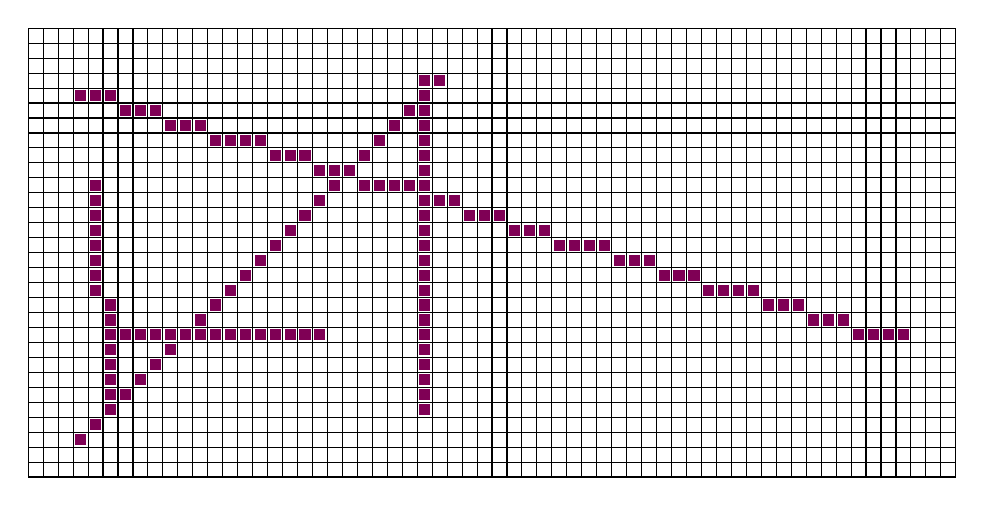
\begin{tikzpicture}[scale=0.19]

  \newcommand{\p}[2]{\node[anchor=center] at (#1 + 0.5, 29 - #2 + 0.5) {{\color{eclipsePurple}\rule{0.4em}{0.4em}}};}

  \begin{scope}
    \draw (0, 0) grid (62, 30);
%
 \p{58}{20}
 \p{57}{20}
 \p{56}{20}
 \p{55}{20}
 \p{54}{19}
 \p{53}{19}
 \p{52}{19}
 \p{51}{18}
 \p{50}{18}
 \p{49}{18}
 \p{48}{17}
 \p{47}{17}
 \p{46}{17}
 \p{45}{17}
 \p{44}{16}
 \p{43}{16}
 \p{42}{16}
 \p{41}{15}
 \p{40}{15}
 \p{39}{15}
 \p{38}{14}
 \p{37}{14}
 \p{36}{14}
 \p{35}{14}
 \p{34}{13}
 \p{33}{13}
 \p{32}{13}
 \p{31}{12}
 \p{30}{12}
 \p{29}{12}
 \p{28}{11}
 \p{27}{11}
 \p{26}{11}
 \p{25}{10}
 \p{24}{10}
 \p{23}{10}
 \p{22}{10}
 \p{21}{9}
 \p{20}{9}
 \p{19}{9}
 \p{18}{8}
 \p{17}{8}
 \p{16}{8}
 \p{15}{7}
 \p{14}{7}
 \p{13}{7}
 \p{12}{7}
 \p{11}{6}
 \p{10}{6}
 \p{9}{6}
 \p{8}{5}
 \p{7}{5}
 \p{6}{5}
 \p{5}{4}
 \p{4}{4}
 \p{3}{4}
 \p{27}{3}
 \p{26}{4}
 \p{25}{5}
 \p{24}{6}
 \p{23}{7}
 \p{22}{8}
 \p{21}{9}
 \p{20}{10}
 \p{19}{11}
 \p{18}{12}
 \p{17}{13}
 \p{16}{14}
 \p{15}{15}
 \p{14}{16}
 \p{13}{17}
 \p{12}{18}
 \p{11}{19}
 \p{10}{20}
 \p{9}{21}
 \p{8}{22}
 \p{7}{23}
 \p{6}{24}
 \p{5}{25}
 \p{4}{26}
 \p{3}{27}
 \p{5}{20}
 \p{6}{20}
 \p{7}{20}
 \p{8}{20}
 \p{9}{20}
 \p{10}{20}
 \p{11}{20}
 \p{12}{20}
 \p{13}{20}
 \p{14}{20}
 \p{15}{20}
 \p{16}{20}
 \p{17}{20}
 \p{18}{20}
 \p{19}{20}
 \p{4}{10}
 \p{4}{11}
 \p{4}{12}
 \p{4}{13}
 \p{4}{14}
 \p{4}{15}
 \p{4}{16}
 \p{4}{17}
 \p{5}{18}
 \p{5}{19}
 \p{5}{20}
 \p{5}{21}
 \p{5}{22}
 \p{5}{23}
 \p{5}{24}
 \p{26}{25}
 \p{26}{24}
 \p{26}{23}
 \p{26}{22}
 \p{26}{21}
 \p{26}{20}
 \p{26}{19}
 \p{26}{18}
 \p{26}{17}
 \p{26}{16}
 \p{26}{15}
 \p{26}{14}
 \p{26}{13}
 \p{26}{12}
 \p{26}{11}
 \p{26}{10}
 \p{26}{9}
 \p{26}{8}
 \p{26}{7}
 \p{26}{6}
 \p{26}{5}
 \p{26}{4}
 \p{26}{3}
  \end{scope}

\end{tikzpicture}
\end{document}
  \end{center}
\caption{Points Generated by the Line Drawing Example.}
\label{fig:lines}
\end{figure}

\begin{enumerate}
\item pseudo random numbers and sobol
\item trees
\item graphs
\item histograms
\item parenthesis matching
\end{enumerate}

%\chapter{Bigger Applications}
%\begin{enumerate}
%\item monte carlo
%\item learning with stochastic gradient descent
%\item stencils
%\item convolutions
%\end{enumerate}

\chapter{Interoperability}
\label{chap:interoperability}

\begin{enumerate}
\item python and c
\item examples: mandelbrot, life, cam, nbody
\end{enumerate}

\bibliographystyle{plain}
\bibliography{bib}

\appendix

\part{Appendices}

\chapter{Tool References}
\begin{enumerate}
\item futhark-c, futhark-opencl
\item measuring runtimes, debugging
\end{enumerate}

\end{document}

%%% Local Variables:
%%% mode: latex
%%% TeX-master: t
%%% End:
